\documentclass[a4paper,leqno,twocolumn]{article}
% ==== Inputs and Usepackages ====

\usepackage{tablefootnote}
\usepackage{enumerate}
\usepackage{float}
\usepackage{url}
\usepackage{hyperref}
\usepackage{dsfont}
\usepackage{mathrsfs}
\usepackage{amsmath}
\usepackage{amssymb}
\usepackage{amsthm}
\usepackage{amsfonts}
\usepackage{mathtools}
%\usepackage{mathabx}
\usepackage{MnSymbol}
\usepackage{xfrac}
\usepackage{nicefrac}
\usepackage{geometry}
\usepackage{graphicx}
\usepackage{graphics}
\usepackage{latexsym}
\usepackage{setspace}
\usepackage{tikz-cd}
\usepackage{tikz}
 \usetikzlibrary{matrix}
 \usetikzlibrary{calc}
 \usetikzlibrary{circuits.ee.IEC}
\usepackage{circuitikz}

\usepackage{a4wide}
\usepackage{fancybox}
\usepackage{fancyhdr}
\usepackage[utf8]{inputenc}




% ==== Page Settings ====

\hoffset = -1.2 in
\voffset = -0.3 in
\textwidth = 590pt
\textheight = 770pt
\setlength{\headheight}{20pt}
\setlength{\headwidth}{590pt}
\marginparwidth = 0 pt
\topmargin = -0.75 in
\setlength{\parindent}{0cm}


% ==== Presettings for files ====

\pagestyle{fancy}


\cfoot{\thepage}
\lfoot{\href{mailto:szekerb@student.ethz.ch}{szekerb@student.ethz.ch}}
\rfoot{Balázs Szekér, \today}
\lhead{Physics \uproman{3} Summary}

% ==== General Commands ====

\newcommand{\sframebox}[1]{
        \framebox[500pt][l]{\parbox{490pt}{
            #1
        }
    }

}

\newcommand{\cframebox}[2]{
        \fbox{\parbox{#1pt}{
            #2
        }
    }
}









% ====== Maths ======


% ==== Formats ====
\newcommand{\boldline}[1]{\textbf{\underline{#1}}}
\newcommand{\uproman}[1]{\uppercase\expandafter{\romannumeral#1}}
\newcommand{\lowroman}[1]{\romannumeral#1\relax}
\newcommand{\fat}[1]{\textbf{#1}}
\newcommand{\Loesung}{\begin{center}\textbf{Lösung}\end{center}}

\newcommand{\Korollar}[1]{\textbf{Korollar} \vspace{1\baselineskip} #1}
\newcommand{\Beispiel}[1]{\textbf{Beispiel} \vspace{1\baselineskip} #1}
\newcommand{\Beweis}[1]{\textbf{Beweis} \vspace{1\baselineskip} #1}
\newcommand{\Proposition}[1]{\textbf{Proposition} \vspace{1\baselineskip} #1}
\newcommand{\Satz}[1]{\textbf{Satz} \vspace{1\baselineskip} #1}
\newcommand{\Definition}[1]{\textbf{Definition} \vspace{1\baselineskip} #1}
\newcommand{\Lemma}[1]{\textbf{Lemma}\vspace{1\baselineskip} #1}
\newcommand{\Bemerkung}[1]{\textbf{Bemerkung} \vspace{1\baselineskip} #1}
\newcommand{\Theorem}[1]{\textbf{Theorem} \vspace{1\baselineskip} #1}




% ==== mathsymbols ====
\newcommand{\Q}{\mathbb{Q}}
\newcommand{\R}{\mathbb{R}}
\newcommand{\N}{\mathbb{N}}
\newcommand{\Z}{\mathbb{Z}}
\newcommand{\C}{\mathbb{C}}
\newcommand{\K}{\mathbb{K}}
\newcommand{\eS}{\mathbb{S}}
\newcommand{\X}{$X$ }
\newcommand{\Y}{$Y$ }
\newcommand{\x}{$x$ }
\newcommand{\y}{$y$ }
\newcommand{\B}{\mathcal{B}}
\newcommand{\A}{\mathcal{A}}
\renewcommand{\S}{\mathcal{S}}
\renewcommand{\P}{\mathcal{P}}



% ==== math operators ====
\newcommand{\klammer}[1]{\left( #1 \right)} 
\newcommand{\eckigeklammer}[1]{\left[ #1 \right]}
\newcommand{\geschwungeneklammer}[1]{\left\{ #1 \right\}}
\newcommand{\floor}[1]{\left\lfloor #1 \right\rfloor}
\newcommand{\ceil}[1]{\left\lceil #1 \right\rceil}
\newcommand{\scalprod}[2]{\left\langle #1 , #2 \right\rangle}
\newcommand{\abs}[1]{\left\vert #1 \right\vert} 
\newcommand{\Norm}[1]{\left\vert\left\vert #1 \right\vert\right\vert}
\newcommand{\intab}{\int_a^b}
\newcommand{\intii}{\int_{-\infty}^\infty} 
\newcommand{\cint}[2]{\int_{#1}^{#2}}
\newcommand{\csum}[2]{\sum_{#1}^{#2}}
\newcommand{\limes}[1]{\lim\limits_{#1}}
\newcommand{\limessup}[1]{\limsup\limits_{#1}}
\newcommand{\limesinf}[1]{\liminf\limits_{#1}}
\newcommand{\limesninf}{\limes{n \rightarrow \infty}}
\newcommand{\limsupninf}{\limessup{n \rightarrow \infty}}
\newcommand{\liminfninf}{\limesinf{n \rightarrow \infty}}
\newcommand{\standardNorm}{\Norm{ \ \cdot \ }}
\newcommand{\einsNorm}{\Norm{ \ \cdot \ }_1}
\newcommand{\zweiNorm}{\Norm{ \ \cdot \ }_2}
\newcommand{\Hom}{\text{Hom}}
\newcommand{\Mat}{\text{Mat}}
\newcommand{\grad}{\text{grad}}
\newcommand{\vol}{\text{vol}}
\newcommand{\supp}{\text{supp}}
\newcommand{\rot}{\text{rot}}
\renewcommand{\div}{\text{div}}



% ==== Analysis ====
\newcommand{\supremum}{\text{sup}}
\newcommand{\infimum}{\text{inf}}
\newcommand{\maximum}{\text{max}}
\newcommand{\minimum}{\text{min}}

\newcommand{\xinX}{$x \in X$ }
\newcommand{\yinY}{$y \in Y$ }
\newcommand{\xyinX}{$x,y \in X$ }
\newcommand{\yinX}{$y \in X$ }
\newcommand{\xinR}{$x \in \R$ }
\newcommand{\xyinR}{$x,y \in \R$ }
\newcommand{\zinC}{$z \in \C$ }
\newcommand{\ninN}{$n \in \N$ }
\newcommand{\NinN}{$N \in \N$}
\newcommand{\angeordneterK}{$(K,\leq)$ }
\newcommand{\xFolge}{(x_n)_{n=0}^{\infty}}
\newcommand{\yFolge}{(y_n)_{n=0}^{\infty}}
\newcommand{\zFolge}{(z_n)_{n=0}^{\infty}}
\newcommand{\aFolge}{(a_n)_{n=0}^{\infty}}
\newcommand{\fFolge}{(f_n)_{n=0}^{\infty}}

\newcommand{\XsubR}{$X \subset \R$ }
\newcommand{\XsubeqR}{$X \subseteq \R$ }

\newcommand{\XFam}{\mathcal{X}}
\newcommand{\PFam}{\mathcal{P}}

\newcommand{\offenesintervall}[2]{$\left( #1 , #2 \right)$ }
\newcommand{\abgeschlossenesintervall}[2]{$\left( #1 , #2 \right)$ }

\newcommand{\XTopRaum}{(X,\tau)}


% ==== Lineare Algebra ====
\newcommand{\vinV}{$v \in V$ }
\newcommand{\uinU}{$u \in U$ }
\newcommand{\winW}{$w \in W$ }
\newcommand{\vwinV}{$v,w \in V$ }

\newcommand{\BasisV}{v_1 , \dots , v_n}
\newcommand{\BasisU}{u_1 , \dots , u_n}
\newcommand{\BasisW}{w_1 , \dots , w_n}

\newcommand{\transpose}[1]{#1^t}
\newcommand{\inverse}[1]{#1^{-1}}
\newcommand{\ddvec}[3]{\left( #1,#2,#3 \right)}
\newcommand{\tdvec}[2]{\left( #1 , #2 \right)}

\newcommand{\Edrei}{\begin{pmatrix}
    1 & 0 & 0 \\
    0 & 1 & 0 \\
    0 & 0 & 1
\end{pmatrix}}

\newcommand{\id}{\text{id}}
\newcommand{\GL}{\text{GL}}
\newcommand{\End}{\text{End}}
\renewcommand{\Im}{\text{Im}}
\renewcommand{\Re}{\text{Re}}
\renewcommand{\ker}{\text{Ker}}
\newcommand{\rang}{\text{rang}}
\newcommand{\ad}{\text{ad}}
\newcommand{\Eig}{\text{Eig}}
\newcommand{\Bil}{\text{Bil}}
\newcommand{\sign}{\text{sign}}
\newcommand{\tr}{\text{tr}}



% ====== Physics ======

% ==== Physicssymbols ====
\newcommand{\epsilonnull}{\epsilon_0}
\newcommand{\munull}{\mu_0}
\newcommand{\rn}{r_0}
\newcommand{\Rn}{R_0}
\newcommand{\rhonull}{\rho_0}
\newcommand{\Rhonull}{\varrho_0}


% ==== Notation ====
\newcommand{\Etot}{E_{\text{Tot}}}
\newcommand{\Wtot}{W_{\text{Tot}}}
\newcommand{\Ftot}{F_{\text{Tot}}}
\newcommand{\vtot}{v_{\text{Tot}}}
\newcommand{\atot}{a_{\text{Tot}}}
\newcommand{\mtot}{m_{\text{Tot}}}
\newcommand{\Mtot}{M_{\text{Tot}}}

\newcommand{\Ekin}{E_{\text{Kin}}}
\newcommand{\Epot}{E_{\text{Pot}}}
\newcommand{\Edef}{E_{\text{Def}}}

\newcommand{\Fg}{F_g}
\newcommand{\FN}{F_N}
\newcommand{\Fz}{F_z}
\newcommand{\FC}{F_C}

\newcommand{\xn}{x_0}
\newcommand{\xN}{x_n}
\newcommand{\vn}{v_0}
\newcommand{\vN}{v_n}
\newcommand{\an}{a_0}
\newcommand{\aN}{a_n}

\newcommand{\dt}{\Delta t}
\newcommand{\dx}{\Delta x}
\newcommand{\dv}{\Delta v}
\newcommand{\da}{\Delta a}
\newcommand{\dE}{\Delta E}
\newcommand{\dW}{\Delta W}
\newcommand{\dF}{\Delta F}


% ==== Relativity ====
\newcommand{\relsqrt}{\sqrt{1-\frac{v^2}{c^2}}}
\newcommand{\relgamma}{\frac{1}{\relsqrt}}


% ==== Constants ====
\newcommand{\g}{9.81}





\renewcommand{\epsilon}{\varepsilon}
\clubpenalty = 10000
\widowpenalty = 10000
\usepackage[skins,theorems]{tcolorbox}

\begin{document}

\tcbset{highlight math style={enhanced, sharp corners=uphill,
  colframe=red!75!black,colback=red!5!white,arc=0pt,boxrule=1pt}}


\section{Quadratur}


\fat{Quadratur} {

    Das Integral wird durch eine gewichtete Summe von der Funktion $f$ an verschiedenen
    Stellen $c_i^n$ angenommenen Werte approximiert:
    \begin{align*}
        \intab f(x) dx \approx Q_n (f;a,b) := \sum_i^n \omega_i^n f(c_i^n)
    \end{align*}
    Hierbei sind die $\omega_i^n$ die \fat{Gewichte} und die $c_i^n \in [a,b]$ die
    \fat{Knoten} der Quadraturformel.
}

\vspace{1\baselineskip}

\fat{Fehler}{

    Der Fehler einer Quadraturformel $Q_n (f)$ ist
    \begin{align*}
        E(n) := \abs{\intab f(x) dx - Q_n (f;a,b)}
    \end{align*}
}

\vspace{1\baselineskip}

\Definition{

    Eine Quadraturformel besitzt \fat{Ordnung} $n+1$, wenn sie Polynome vom Grad $n$ exakt
    integriert.
}

\vspace{1\baselineskip}

\fat{Mittelpunkt-Regel} {
    \begin{align*}
        Q^M (f;a,b) = (b-a) f\klammer{\frac{a+b}{2}}
    \end{align*}
    Sie besitzt Ordnung $2$.
}

\vspace{1\baselineskip}

\fat{Trapezregel} {

    Quadraturformel der Ordnung $2$.
    \begin{align*}
        Q^T (f;a,b) = \frac{b-a}{2} (f(a)+f(b))
    \end{align*}
    Für den Fehler gilt:
    \begin{align*}
        E(n) = \abs{- \frac{1}{12} (b-a)^3 f^{(2)} (\xi)}
    \end{align*}
    mit einem $\xi \in [a,b]$.
}

\vspace{1\baselineskip}

\fat{Simpson-Regel} {
    
    Quadraturformel der Ordnung $4$. Bedarf drei Stützstellen:
    \begin{align*}
        Q^s (f;a,b) = \frac{b-a}{6} \klammer{f(a)+4 f\klammer{\frac{a+b}{2}} + f(b)}
    \end{align*}
    Der Fehler ist:
    \begin{align*}
        E(n) = \abs{-\frac{1}{90} \klammer{\frac{b-a}{2}}^5 f^{(4)} (\xi)}
    \end{align*}
    mit einem $\xi \in [a,b]$
}

\vspace{1\baselineskip}

\fat{Summierte Mittelpunkt-Regel} {
    \begin{align*}
        I(f;a,b) \approx \sum_{i=0}^{N-1} h f \klammer{\frac{x_i + x_{i+1}}{2}}
    \end{align*}
    Mit $h=\frac{b-a}{2}$, $x_0 = a$, $x_i = x_0 + i h$, $x_N = b$.
}

\vspace{1\baselineskip}

\fat{Summierte Trapezregel} {
    \begin{align*}
        I(f;a,b) \approx& \sum_{i=0}^{N-1} \frac{h}{2} (f(x_i) + f(x_{i+1})) \\
        &= \frac{h}{2} \klammer{f(a) + 2 \sum_{i=1}^{N-1} f(x_i) + f(b)}
    \end{align*}
    Mit $h=\frac{b-a}{2}$, $x_0 = a$, $x_i = x_0 + i h$, $x_N = b$.
}

\vspace{1\baselineskip}

\fat{Summierte Simpson-Regel} {
    \begin{align*}
        I(f;a,b) \approx& \sum_{i=0}^{N-1} \frac{h}{6} \klammer{f(x_i) +
            4 f\klammer{\frac{x_i + x_{i+1}}{2}} + f(x_{i+1})}
        \\
        &=\frac{h}{6} \klammer{f(a) + 2 \sum_{i=1}^{N-1} f(x_i) + 4 \sum_{i=1}^N f \klammer{\frac{x_{i-1} + x_i}{2}} + f(b)}
    \end{align*}
    Mit $h=\frac{b-a}{2}$, $x_0 = a$, $x_i = x_0 + i h$, $x_N = b$.
}

\vspace{1\baselineskip}

\fat{Gauss-Legendre Quadratur} {

    \begin{itemize}
        \item $n=2$:
            \begin{align*}
                \int_{-1}^1 f(x) dx \approx Q_2^G =
            2 \cdot \klammer{\frac{1}{2} f \klammer{\frac{-1}{\sqrt{3}}} + \frac{1}{2} f \klammer{\frac{1}{\sqrt{3}}}}
            \end{align*}
        \item $n=3$:
            \begin{align*}
                \int_{-1}^1 f(x) dx \approx Q_3^G =
            2 \cdot \klammer{\frac{5}{18} f \klammer{\frac{- \sqrt{15}}{5}} + \frac{8}{18} f(0) + \frac{5}{18} f \klammer{\frac{\sqrt{15}}{5}}}
            \end{align*}
        \item Allgemeine $n$:
            \begin{align*}
                \int_{-1}^1 f(x) dx \approx 2 \cdot \sum_{i=1}^n w_i f(c_i)
            \end{align*}
            Die Stützstellen $c_i$ sind die EW der Matrix:
            \begin{align*}
                \begin{pmatrix}
                    0 & b_1 & & & \\
                    b_1 & 0 & b_2 & & \\
                    & b_2 & \ddots & \ddots & \\
                    & & \ddots & \ddots & b_{n-1} \\
                    & & & b_{n-1} & 0
                \end{pmatrix}
                \quad \text{ mit } \quad
                b_j = \frac{j}{\sqrt{4 j^2 -1}}                
            \end{align*}
    \end{itemize}
    
    \begin{center}
        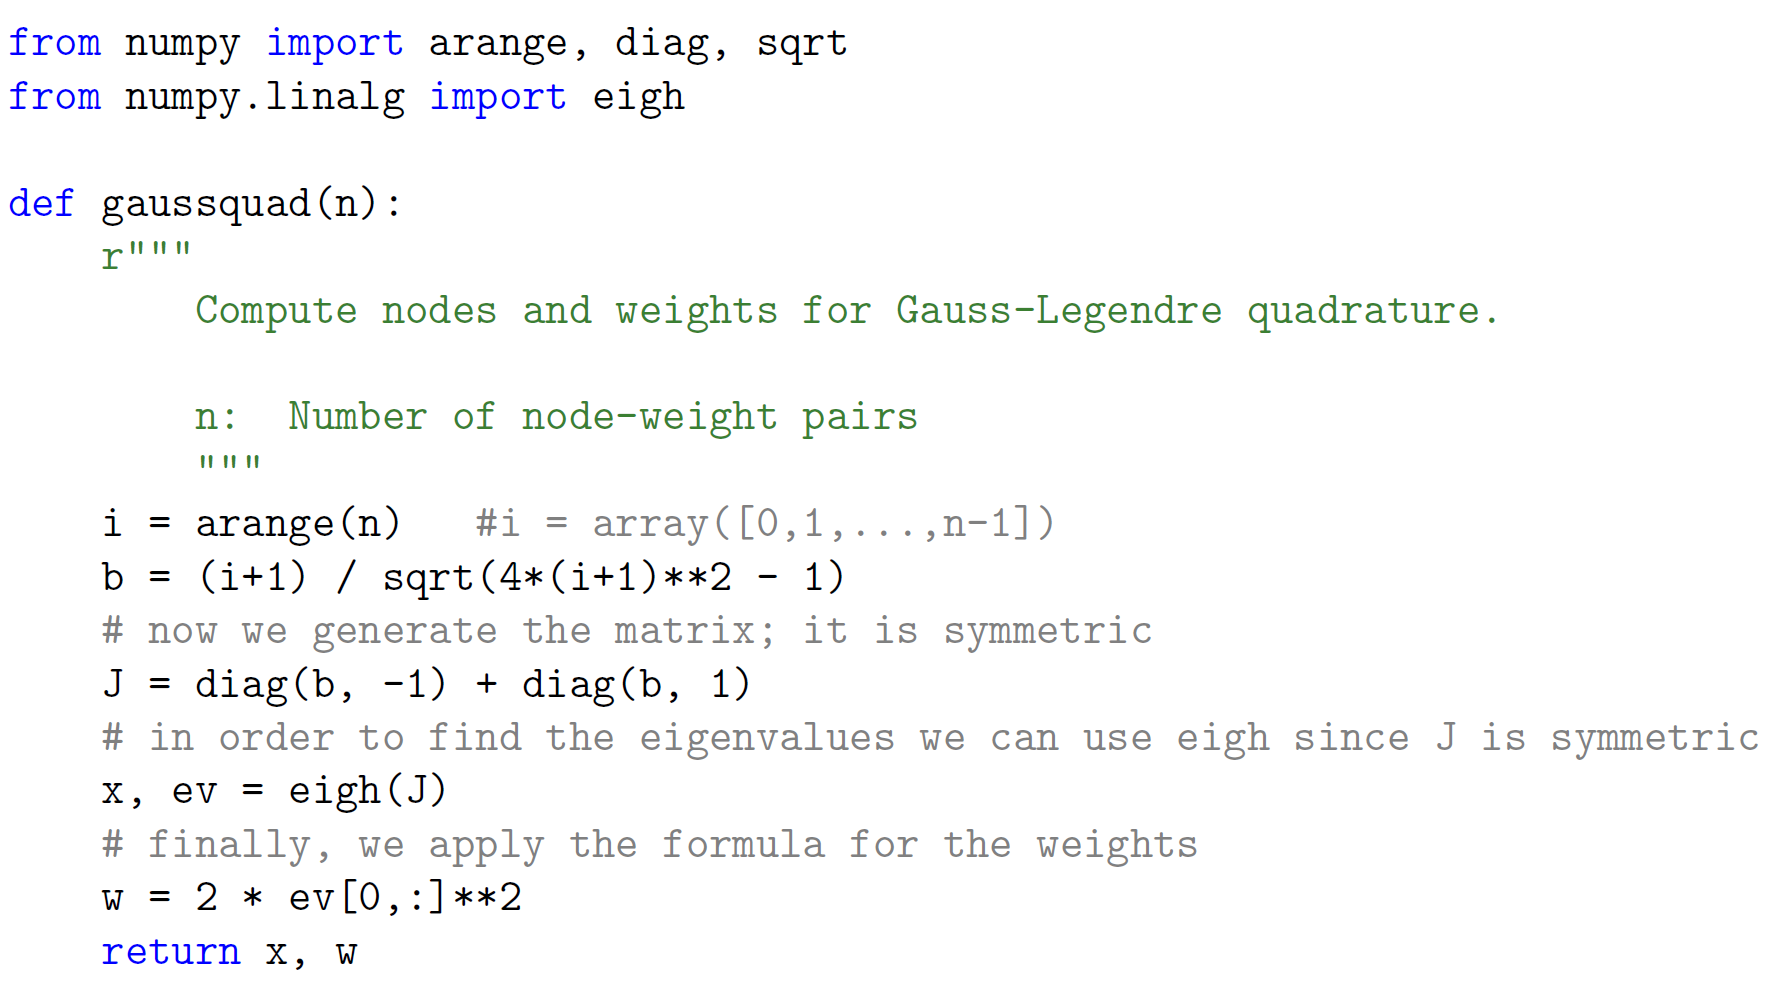
\includegraphics[width=0.3\textwidth]{Figures/Gauss_Legegendre.png}

        Skript Seite 16
    \end{center}    
}

\vspace{1\baselineskip}

\fat{Clenshaw-Curtis Formel} {

    Wir substituieren:
    \begin{align*}
        \int_{-1}^1 f(x) dx = \int_0^{\pi} f(\cos(\theta)) \sin(\theta) d \theta
        = \sum_{\text{k gerade}} \frac{2 a_k}{1-k^2}
    \end{align*}

    \begin{center}
        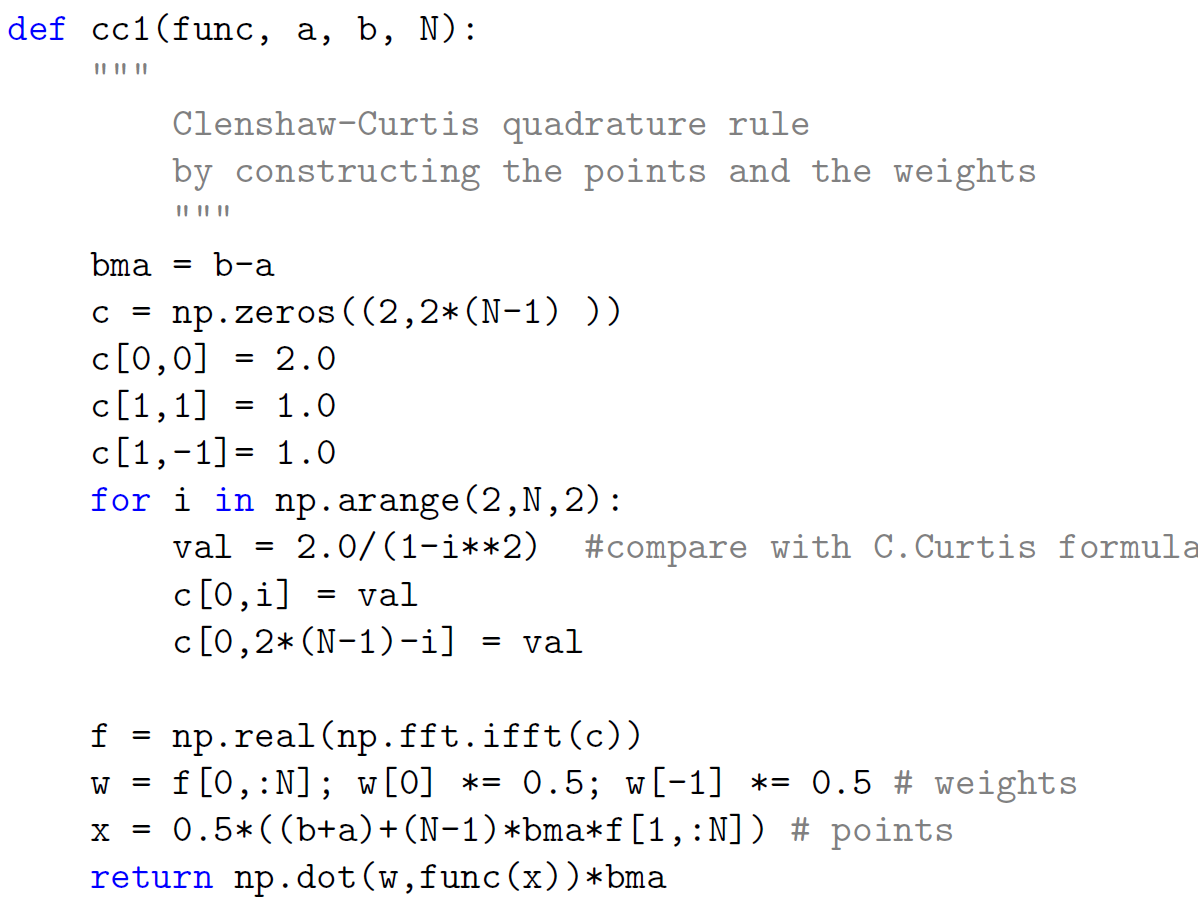
\includegraphics[width=0.4\textwidth]{Figures/cc1.png}

        Skript Seite 18
    \end{center}
    

    \begin{center}
        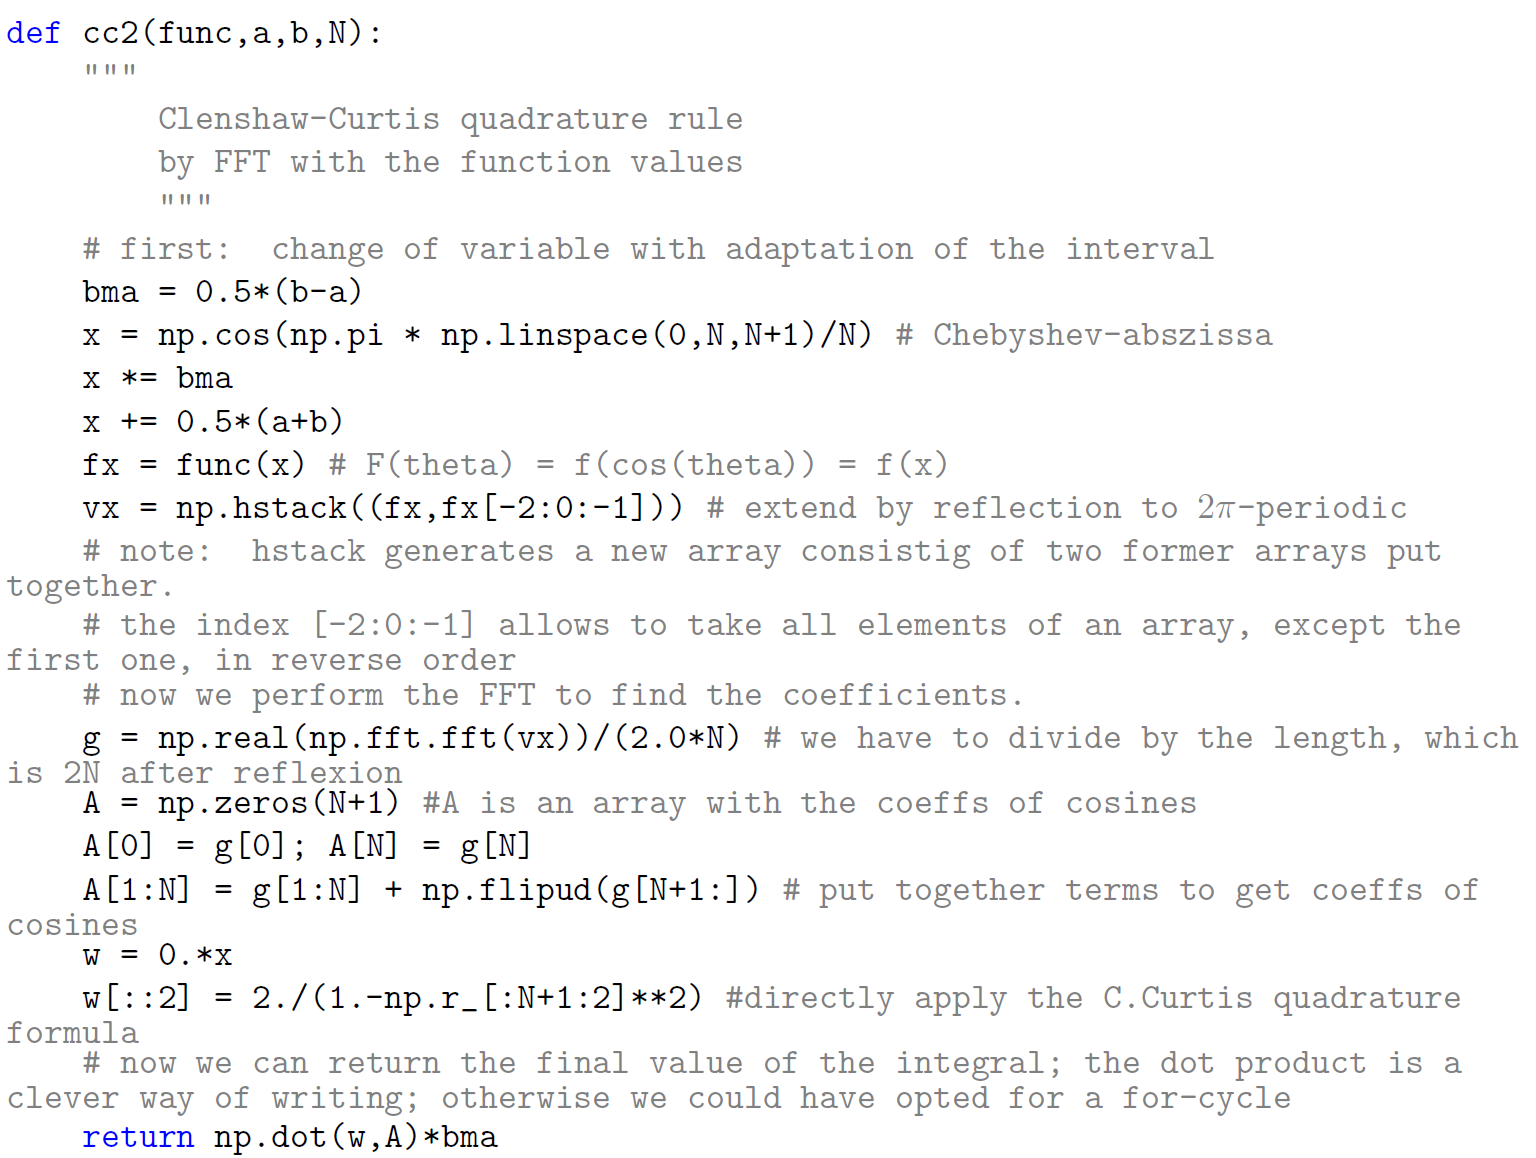
\includegraphics[width=0.5\textwidth]{Figures/cc2.png}

        Skript Seite 17
    \end{center}
}

\vspace{1\baselineskip}

\fat{Adaptive Quadratur}

    \begin{center}
        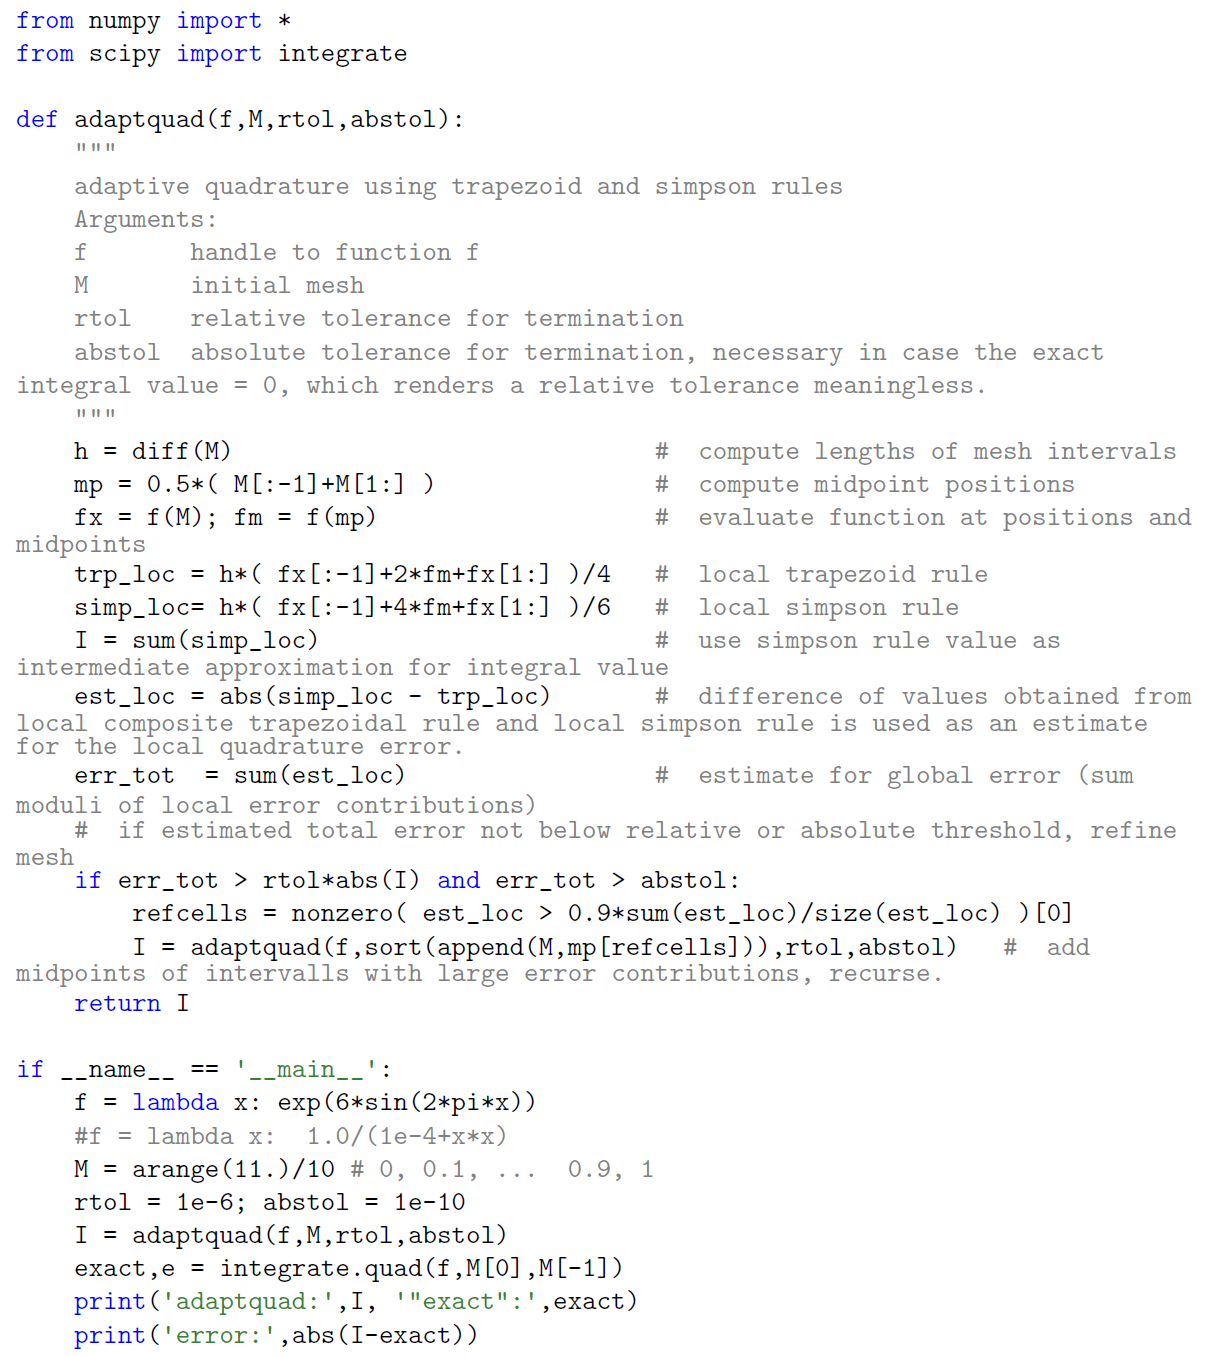
\includegraphics[width=0.4\textwidth]{Figures/AdaptQuad.png}

        Skript Seite 22
    \end{center}


\vspace{1\baselineskip}

\fat{Mehrdimensionale Integration} {

    Mit Satz von Fubini: eins nach dem anderen integrieren:
    \begin{align*}
        \int_{a_1}^{b_1} \dots \int_{a_d}^{b_d} f(x_1,\dots,x_d) dx_1 \dots dx_d
        \\
        \approx \sum_{i_1 = 0}^{n_1} \dots \sum_{i_d = 1}^{n_d} w_{i_1}^1 \dots w_{i_d}^{n_d} f(c_{i_1}^1 , \dots , c_{i_d}^d)
    \end{align*}
}

\vspace{1\baselineskip}

\fat{Python Code}:
\begin{itemize}
    \item Eindimensionale Integration: scipy.integrate.quad(f,a,b)[0]
    \item Mehrdimensionale Integration: 
    
            scipy.integrate.nquad(f,array([[a1,b1],\dots,[ad,bd]]))[0]
\end{itemize}

\vspace{1\baselineskip}

\fat{Drei Term Rekursion der Legendre Polynome}:
\begin{align*}
    P_{k+1} (x) = \klammer{x- \frac{\scalprod{x \cdot P_k}{P_k}}{\scalprod{P_k}{P_k}}} \cdot P_{k} (x)
        -  \klammer{\frac{\scalprod{P_k}{P_k}}{\scalprod{P_{k-1}}{P_{k-1}}}} P_{k-1} (x)
\end{align*}
Mit $P_0 (x) =1$ und $P_{-1} (x) = 0$
 
\vspace{1\baselineskip}

\Definition{

    Wir definieren die \fat{Lagrange-Polynome} für die Stützstellen $x_1,\dots,x_n$
    als
    \begin{align*}
        l_i (x) = \prod_{\stackrel{j=0}{i \neq j}} \frac{x-x_j}{x_i - x_j}
    \end{align*}
    Für diese gelten:
    \begin{enumerate}
        \item $l_i (x_j) = \delta_{ij}$
        \item $\grad \  l_i = n$
        \item $\sum_{i=0}^{n} l_i (x) = 1 \ \forall x \in \R$
        \item $\sum_{i=0}^{n} l_i^{(m)} (x) = 0$ für $m \geq 1$
        \item $l_1,\dots,l_n$ bilden eine Basis im Raum der Polynome von Grad $\leq n$.
    \end{enumerate}
}

\vspace{1\baselineskip}

\fat{Drei Term Rekursion der Lagrange Polynome}
\begin{align*}
    x P_{k-1} (x) = \frac{c_k}{a_k} P_{k-2} (x) - \frac{b_k}{a_k} P_{k-1} (x) + \frac{1}{a_k} P_{k} (x)
\end{align*}
Dies können wir in Matrixform bringen:
\begin{align*}
    A = \begin{pmatrix}
        - \frac{b_1}{a_1} & \frac{1}{a_1} & & & 0 \\
        \frac{c_2}{a_2} & - \frac{b_2}{a_2} & \frac{1}{a_2} & & \\
        & \ddots & \ddots & \ddots & \\
        & & \frac{c_{n-1}}{a_{n-1}} & \frac{b_{n-1}}{a_{n-1}} & \frac{1}{a_{n-1}} \\
        0 & & & \frac{c_n}{a_n} & \frac{b_n}{a_n}
    \end{pmatrix}
\end{align*}
Dies ist die gleiche Matrix wie bei der Gauss-Legendre Quadratur.
Sei $P_A$ das charakteristische Polynom von $A$. Dann sind die NST von $P_A$ die
Knotenpunkte der Gauss-Quadraturformel und die zu den jeweiligen Knotenpunkten
gehörigen Gewichte sind definiert als:
\begin{align*}
    w_j = \frac{1}{\Norm{v_j}}
\end{align*}
mit $v_j$ dem Eigenvektor zum Eigenwert $c_j$. Da diese aber nicht eindeutig sind,
muss normiert werden. Wir finden mit folgendem Verfahren die richtigen Eigenvektoren:
\begin{enumerate}
    \item Schreibe $u_j = c \cdot v_j = c \cdot [P_0 (t_j) , \dots , P_{n-1} (t_j)]^T$ für
            alle Eigenvektoren.
    \item Es muss gelten: $1=\scalprod{P_0}{P_0} = \int_{-1}^1 P_0 (t_1) P_0 (t_1) dx \
            \Longrightarrow P_0 (t_1) = \frac{1}{\sqrt{2}}$
    \item Wir betrachten den ersten Eintrag vom Eigenvektor: $(v_j)_1 = c \cdot P_0 (t_1) =
            c \cdot \frac{1}{\sqrt{2}} \ \Longrightarrow c = \sqrt{2} (v_j)_1$
    \item Man normiere alle Eigenvektoren: $v_j = \frac{1}{c} u_j = \frac{1}{\sqrt{2} (v_j)_1}
            v_j$
    \item Zum Schluss: $w_j = \frac{2 (v_j)_1^2}{\Norm{v_j}^2}$
\end{enumerate}



\vspace{1\baselineskip}

\section{Gewöhnliche DGL}

\vspace{1\baselineskip}

\Definition{

    Eine gewöhnliche DGL heisst \fat{autonom}, wenn $f$ unabhängig von $t$ ist.
}

\vspace{1\baselineskip}

\fat{Umwandlung in DGL erster Ordnung}

Gegeben: $\vec{y}_n = \vec{f} \klammer{t,\vec{y},\dots,\vec{y}^{(n-1)}}$

Vorgehen:
\begin{enumerate}
    \item Schreibe einen Vektor mit Einträgen $\vec{y}(t),\dots,\vec{y}^{(n-1)}(t)$:
            $$
                \vec{z}(t) = \begin{pmatrix}
                    \vec{z_0} \\ \vdots \\ \vec{z}_{n-1} (t)
                \end{pmatrix}
                := \begin{pmatrix}
                    \vec{y} (t) \\ \vdots \\ \vec{y}^{(n-1)}
                \end{pmatrix}
            $$
    \item Leite diesen Vektor ab und setze die DGL ein:
            $$
                \frac{d}{dz} \vec{z} (t) = \begin{pmatrix}
                    \vec{y}' \\ \vdots \\ \vec{y}^{(n)} (t)
                \end{pmatrix} = \begin{pmatrix}
                    \vec{z}_1 (t) \\ \vdots \\ \vec{y}^{(n-1)} (t) \\ \vec{f}(t,\vec{y},\dots,\vec{y}^{(n-1)})
                \end{pmatrix}
                =: \vec{g}(t,\vec{z})
            $$
\end{enumerate}

\vspace{1\baselineskip}

\fat{Autonomisierung einer DGL}

Hat man eine DGL erster Ordnung $\dot{\vec{y}} = \vec{f}(t,\vec{y})$ mit $\vec{y} \in \R^n$,
so kann man di Zeitabhängigkeit in die DGL einpacken. Das Vorgehen ist genau analog zur
Umwandlung in eine DGL erster Ordnung. Dazu wird $\vec{z} \in \R^{n+1}$ eingeführt:
$$
    \vec{z} (t) := \begin{pmatrix}
        \vec{y} (t) \\ t
    \end{pmatrix}
    =
    \begin{pmatrix}
        \vec{z} \\ z_{n+1}
    \end{pmatrix}
$$
Somit erhalten wir die autonome DGL:
$$
    \dot{\vec{z}} (t) = \begin{pmatrix}
        \vec{f} (z_{n+1} , \vec{z}) \\ 1
    \end{pmatrix}
    =: \vec{g} (\vec{z})
$$

\vspace{1\baselineskip}

\fat{Konvergenzordnung}

Sei $p > 0$ die Konvergenzordnung des Verfahrens sodass $\forall N \in \N \ : \
E(N) \leq \frac{c}{N^p}$ bzw $E(h) \leq c h^p$ mit $h:= \frac{t_{\text{end}} - t_{0}}{N}$
und einer Konstanten $c$. Berechnung: $E(N) \approx c N^{-p} \Leftrightarrow
\log(E(N)) \approx \log(c) - p \log(N)$ $\Leftrightarrow$ Plot von $E$ gegen $N$ in einem
LogLog-Plot ist eine Gerade mit Steigung $-p$

\vspace{1\baselineskip}

\fat{Vorgehen} (Bestimmung der Konvergenzordnung)

- Verwende das Verfahren und löse die DGL mehrmals für verschiedene $N$.

- Berechne für jedes $N$: $e(N) := \Norm{\vec{y}_{\text{exact}} - \vec{y}_N}$

- Berechne:

$p = - \text{polyfit} (\log(N) , \log(e), 1)[0] = \text{polyfit} (\log(h),\log(e),1)[0]$

\vspace{1\baselineskip}

\underline{\fat{Polygonzugverfahren}}

Gegeben: $\dot{\vec{y}} = \vec{f}(t,\vec{y})$, $\vec{y}(t_0) = \vec{y}_0$

Gesucht: Lösung $y(t)$ des AWP 1. Ordnung

\vspace{1\baselineskip}

\fat{Explizites Eulerverfahren}

Approximation durch Tangende zum Anfangszeitpunkt $t_k$.

$\vec{y}_{k+1} := \vec{y}_k + h_k \vec{f}(t_k,\vec{y}_k)$

Lokaler Fehler: $O(h^2)$

\begin{center}
    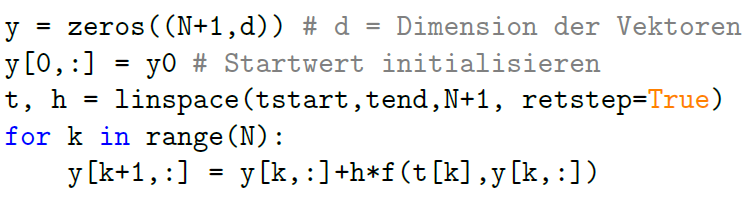
\includegraphics[width=0.3\textwidth]{Figures/eE.png}
\end{center}

\vspace{1\baselineskip}

\fat{Implizites Eulerverfahren}

Approximation durch Tangente am nächsten Zeitpunkt $t_{k+1}$.

$\vec{y}_{k+1} := \vec{y}_k + h_k \vec{f}(t_{k+1} , \vec{y}_{k+1})$

$\Rightarrow \vec{y}_{k+1}$ NST von: $F(\vec{X}) := \vec{X} - \vec{y}_k - h_k \vec{f}(t_{k+1},\vec{X})$


Guter Startwert für Nullstellensuche: Schritt aus eE

Implizit bedeutet, dass für $\vec{y}_{k+1}$ eine (i.A. nichtlineare) Gleichung aufgelöst
werden muss.

Lokaler Fehler: $O(h^2)$

\begin{center}
    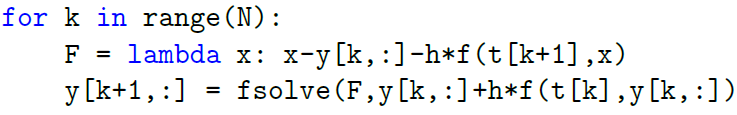
\includegraphics[width=0.31\textwidth]{Figures/iE.png}
\end{center}

\vspace{1\baselineskip}

\fat{Implizite Mittelpunktregel}

Approximation durch Tangente zum Zeitpunkt $(t_k + t_{k+1})/2$

$\vec{y}_{k+1} := \vec{y}_k + h_k \vec{f}(\frac{1}{2}(t_k+t_{k+1}),\frac{1}{2}(\vec{y}_k + \vec{y}_{k+1}))$

$\Rightarrow \vec{y}_{k+1}$ NST von: $F(\vec{X}) := \vec{X} - \vec{y}_k - h_k \vec{f}(\frac{1}{2}(t_k + t_{k+1}),\frac{1}{2}(\vec{y}_k + \vec{X}))$

Guter Startwert für Nullstellensuche: Schritt aus eE

\vspace{1\baselineskip}

Lokaler Fehler: $O(h^3)$

\begin{center}
    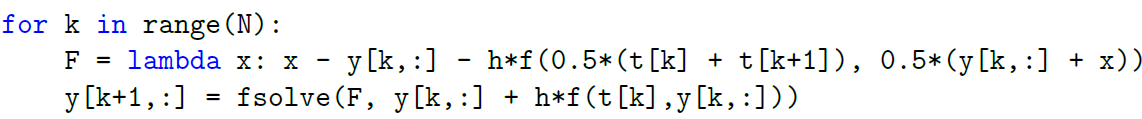
\includegraphics[width=0.48\textwidth]{Figures/iM.png}
\end{center}

\vspace{1\baselineskip}

\fat{Implizite Trapezregel}

$\vec{y}_{k+1} = \vec{y}_k + \frac{h}{2} \klammer{\vec{f}(t_k,\vec{y}_k) + \vec{f}(t_{k+1} , \vec{y}_{k+1})}$

$\Rightarrow y_{k+1}$ NST von: $F(\vec{X}) = \vec{X} - \vec{y}_k - \frac{h}{2} \klammer{\vec{f}(t_k,\vec{y}_k) + \vec{f}(t_{k+1} , \vec{X})}$

Guter Startwert für Nullstellensuche: Schritt aus eine

Lokaler Fehler: $O(h^3)$

\vspace{1\baselineskip}

\underline{\fat{Störmer-Verlet-Verfahren}}

Geg.: $\ddot{\vec{y}} = \vec{f}(t,\vec{y})$ (keine $\dot{\vec{y}}$ Abhängigkeit!),
$\vec{y} (t_0) = \vec{y}_0$, $\dot{\vec{y}}(t_0) = \vec{v}_0$

Ges. Lösung $\vec{y}(t)$ des AWP 2. Ordnung

\vspace{1\baselineskip}

\fat{Zwei-Schritt-Verfahren}

Idee: Approximation durch eine Parabel und äquidistante $t_k$

Idee: $f(t_k , y_k) = \ddot{y}_k \approx \frac{\dot{y}_{k+1} - \dot{y}_k}{h} \approx
\frac{\frac{y_{k+1} - y_k}{h} - \frac{y_k - y_{k-1}}{h}}{h} \approx
\frac{y_{k+1} - 2 y_k + y_{k-1}}{h^2}$

$\vec{y}_{k+1} := - y_{k-1} + 2 \vec{y}_k + h^2 \vec{f}(t_k , \vec{y}_k)$

mit zweitem Startwert: $\vec{y}_1 = \vec{y}_0 + h \vec{v}_0 + \frac{h^2}{2} \vec{f}(t_0,\vec{y}_0)$

\begin{center}
    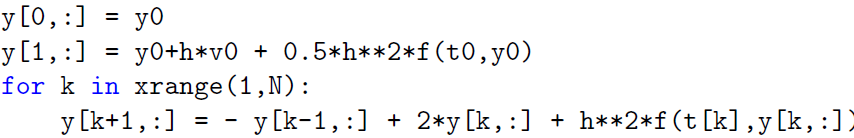
\includegraphics[width=0.35\textwidth]{Figures/ZSF.png}
\end{center}

\vspace{1\baselineskip}

\fat{Ein-Schritt-Verfahren}

Idee: $\ddot{\vec{y}} = \vec{f}(t,\vec{y}) \Leftrightarrow \dot{\vec{y}} = \vec{v}$ und
$\dot{\vec{v}} = \vec{f}(t,\vec{y})$

Verwende das eE für $\dot{\vec{y}}(t) = \vec{v}(t)$ und
$\dot{\vec{v}}(t) = \vec{f}(t,\vec{y})$

Es gibt 2 Methoden: Leap-Frog-Methode und Velocity-Verlet

\vspace{1\baselineskip}

\fat{Leap-Frog-Methode}

$\vec{v}_{k+\frac{1}{2}} := \vec{v}_{k-\frac{1}{2}} + h \vec{f}(t_k,\vec{y}_k)$

$\vec{y}_{k+1} := \vec{y}_k + h \vec{v}_{k+\frac{1}{2}}$

mit Startwert $\vec{v}_{\frac{1}{2}} = \vec{v}_0 + \frac{h}{2} \vec{f}(t_0,\vec{y_0})$

\begin{center}
    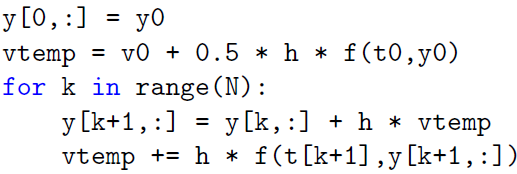
\includegraphics[width=0.2\textwidth]{Figures/ESF.png}
\end{center}

\vspace{1\baselineskip}

\fat{Velocity-Verlet}

$\vec{y}_{k+1} := \vec{y}_k + h \vec{v}_k + \frac{h^2}{2} \vec{f}(t_k,\vec{y}_k)$

$\vec{v}_{k+1} := \vec{v}_k + \frac{h}{2} \klammer{\vec{f}(t_k,\vec{y}_k) + \vec{f}(t_{k+1},\vec{y}_{k+1})}$

\begin{center}
    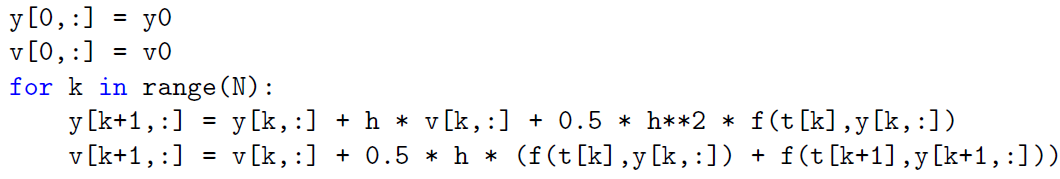
\includegraphics[width=0.4\textwidth]{Figures/VV.png}
\end{center}

Im Gegensatz zu Leap-Frog liefert Vel.Verl. die Geschw. bei $t_k$.

\vspace{1\baselineskip}

Die Einschritt-Verfahren sind numerisch stabiler.

In allen Störmer-Verlet-Verfahren ist die Energie erhalten.

Code im Skript auf Seite 80

\vspace{1\baselineskip}

\fat{Konvergenzordnung}

Wie bei Quadratur.

Exacte Lösung: ode45

from ODE45 import ODE45

$t,y =$ ode45$(f,(t_0,t_{\text{end}}),y_0)$

\vspace{1\baselineskip}

\underline{\fat{Fehler}}
\begin{itemize}
    \item Lokaler Fehler: $\Norm{y(t_{n+1}) - y_{n+1}}$ abschätzen durch fixe Konstanten.
    \item Fehlerfortpflanzung: $\Norm{y_{n+1}^{\star} - y_{n+1}}$ abschätzen mit $y(t_n)$
            und $y_n$.
            Methode: Approximiere $y_{n+1}^{\star}$ mit $y_n$ und $y_{n+1}$ mit $y(t_n)$
    \item Fehlerakkumulierung: Über die Fehlerfortpflanzung bis $n$ summieren. Die Potenz
            nicht vergessen. Tipp: Geometrische Reihe.
\end{itemize}

\vspace{1\baselineskip}

\Theorem{

    $\Norm{\vec{y}_n - \vec{y}(t_n)} \leq M \cdot h$ für alle $n$, wobei

    $M = \frac{1}{L} \klammer{e^{L(T-t_0)} -1} \frac{1}{2} \max \Norm{\ddot{\vec{y}}(t)}$
    \ \ für $t \in [t_0,T]$.

    Kann man mittels den vorherigen drei Fehlertypen beweisen.
}


\vspace{1\baselineskip}

\section{Strukturerhaltung}

\vspace{1\baselineskip}

\Definition{

    Eine Funktion $I : D \rightarrow \R$ heisst \fat{ersts Integral/Invariante} der DGL,
    wenn $I(y(t)) \equiv$ const. für jede Lösung $y=y(t)$ der DGL.
    Eine notwendige und hinreichende Bedingung für differenzierbares erstes Integral der
    DGL ist
    $$
        \grad I(y) f(t,y) = 0 \quad \quad \text{ für alle } (t,y) \in [t_0,T] \times D
    $$
}

\vspace{1\baselineskip}

\Definition{

    Sei $H: \R \times \R \rightarrow \R$ mit $H=H(q,p)$ stetig differenzierbar, dann ist
    das \fat{autonome Hamilton-System} das folgende System von DGL:
    \begin{align*}
        \begin{cases}
            \dot{q_j} = \frac{\partial H}{\partial p_j} (q,p)
            \\
            \dot{p_j}(t) = - \frac{\partial H}{\partial q_j} (q,p)
        \end{cases}
        \quad \quad \text{ für } j=1,2,\dots,d
    \end{align*}
    Die Hamilton Funktion $H$ ist ein erstes Integral des dazugehörigen autonomen
    Hamilton-Systems. Die mehrdimensionale Verallgemeinerung der Hamilton-Systeme lautet:
    \begin{align*}
        \begin{cases}
            \dot{\vec{q}} (t) = \nabla_p H(\vec{q},\vec{p})
            \\
            \dot{\vec{p}} (t) = - \nabla_q H(\vec{q},\vec{p})
        \end{cases}
    \end{align*}
    Zusätzlich kann der Hamiltonian $H(q,p,t)$ explizit von der Zeit abhängen. Die DGL
    bleiben gleich, doch dann ist $H$ nicht mehr erhalten.
}

\vspace{1\baselineskip}

\underline{\fat{Splitting-Verfahren}}

Geg.: AWP 1. Ordnung, autonom: $\dot{\vec{y}} = f(y)$ und $\vec{y}(t_0) = y_0$
das nur schwer oder gar nicht analytisch lösbar ist.

Wenn DGL nicht autonom ist, muss man autonomisieren.

\vspace{1\baselineskip}

\fat{Evolutionsoperatoren}

$\Phi^{t_0,t} : D \subset \R^n \rightarrow D$ heisst Evolutionsoperator zur DGL
$\dot{\vec{y}} = \vec{f}(t,\vec{y})$, wenn $\forall \vec{y}_0 \in D$ gilt:
$\Phi^{t_0 , t} \vec{y}_0 = \vec{y} (t)$ eine Lösung des AWP $\dot{\vec{y}}=\vec{f}(t,\vec{y})$,
$\vec{x}(t_0) = \vec{y}_0$ ist.

Für autonome DGL gilt: $\Phi^{t_0 , t} = \Phi^{0,t-t_0} := \Phi^{t-t_0} := \Phi^h$

Numerische Verfahren liefern den diskreten Evolutionsoperator $\Psi^h \approx \Phi^h$

\vspace{1\baselineskip}

Geg.: Autonome, separierte DGL $\dot{\vec{y}} = \vec{f}_a (\vec{y}) + \vec{f}_b (\vec{y})$,
$\vec{y}(t_0) = \vec{y}_0$

Mit bekannten Evolutionsoperatoren $\Phi_a^h$ zu $\dot{\vec{y}} = \vec{f}_a (\vec{y})$ und
$\Phi_b^h$ zu $\dot{\vec{y}} = \vec{f}_b (\vec{y})$

Ges.: Lösung $\vec{y}(t)$ des AWP 1. Ordnung

Idee: Zerlege ein kompliziertes Problem in zwei Teilprobleme

\vspace{1\baselineskip}

\fat{Lie-Trotter-Splitting}: $\Psi_1^h = \Phi_a^h \circ \Phi_b^h$ oder $\Psi_1^h = \Phi_b^h \circ \Phi_a^b$

\fat{Strange-Splitting}: $\Phi_2^h = \Phi_a^{\nicefrac{h}{2}} \circ \Phi_b^h \circ \Phi_a^{\nicefrac{h}{2}}$

\fat{Allgemein}: $\Psi_s^h = \prod_{i=1}^{s} \Phi_b^{b_i h} \cdot \Phi_a^{a_i h}$ mit
        $\sum_{i=1}^{s} b_i = \sum_{i=1}^{s} a_i = 1$

\vspace{1\baselineskip}

\Bemerkung{

    Das Splittingverfahren kann als Verallgemeinerung des Störmer-Verlet Verfahren
    betrachtet werden. Sind $\Phi_a$ und $\Phi_b$ nicht bekannt, können diskrete
    Evolutionsoperatoren $\Psi_a$ und $\Phi_b$ verwendet werde.
}

\vspace{1\baselineskip}

\fat{Processing}
\begin{align*}
    \hat{\Psi} = \Pi^h \circ \Psi^h \circ \klammer{\Pi^h}^{-1}
\end{align*}
Dabei ist $\Pi^h$ der \fat{post-processor} und $\klammer{\Pi^h}^{-1}$ der \fat{pre-processor}.
Der Vorteil dieser Schreibweise:
\begin{align*}
    \klammer{\hat{\Psi}^h}^n = \Pi^h \circ \klammer{\Psi^h}^n \circ \klammer{\Pi^h}^{-1}
\end{align*}
Vorteile falls:
$\hat{\Psi}^h$ genauer als $\Psi^h$,
$\Pi^h$, $\klammer{\Pi^h}^{-1}$ günstig,
keine/wenige Ausgaben der Lösung vor Endschritt gewünscht.


\vspace{1\baselineskip}

\section{Runge-Kutta-Verfahren}

\vspace{1\baselineskip}

Geg.: $\dot{\vec{y}} = \vec{f}(t,\vec{y})$ wobei $\vec{y} (t_0) = \vec{y}_0$

Ges.: Lösung $\vec{y}(t)$ des AWP 1. Ordnung

Idee: Schreibe das DGLproblem in ein Integrationsproblem um:
$\vec{y}(t_1) = \vec{y}(t_0) + \int_{t_0}^{t_1} \vec{f}(t,\vec{t}) dt$ und verwende eine
Quadraturformel zur Approximation des Integrals:

$\vec{y} (t_1) \approx \vec{y}_0 + h \sum_{i=1}^s b_i \vec{f}(t_0 + c_i h , \vec{y} (t_0 + c_i h))$

mit Gewichten $b_i$ und Stützstellen $c_i \in [0,1]$ und $h=t_1-t_0$

\pagebreak

\fat{Explizite Mittelpunktsregel}

Wir wählen die Mittelpunktsregel als QF. Der noch unbekannte Funktionswert in der
Mitte $y(t_0 + \frac{h}{2})$ wird durch eE approximiert.

\begin{center}
    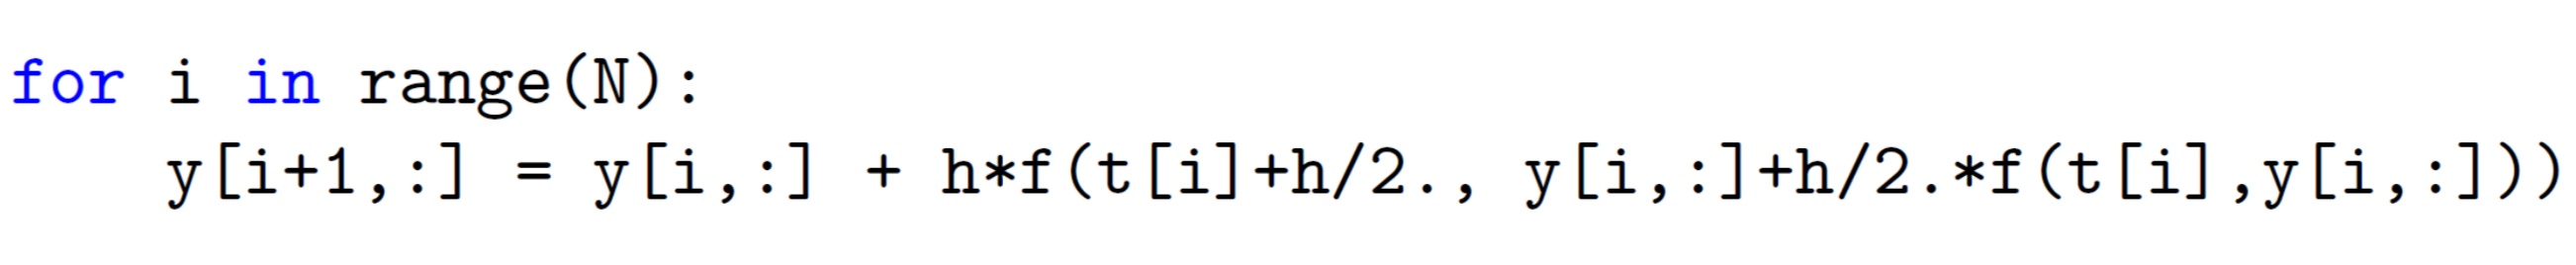
\includegraphics[width=0.45\textwidth]{Figures/RK_eM.png}
\end{center}

Mit der Notation für allgemeine RK Verfahren lässt sich dies schreiben als:
$\vec{k}_1 := \vec{f}(t_0,\vec{y}(t_0))$ und
$\vec{k}_2 := \vec{f}(t_0 + \frac{h}{2} , \vec{y}_0 + \frac{h}{2} \vec{k}_1)$.
Dann ist $\vec{y}_1 = \vec{y}_0 + h \vec{k}_2$.

\vspace{1\baselineskip}

\fat{Explizite Trapezregel}

Wir wählen die Trapezregel als QF. Der noch unbekannte Funktionswert $y(t_0 + h)$ wird
durch eE approximiert.

\begin{center}
    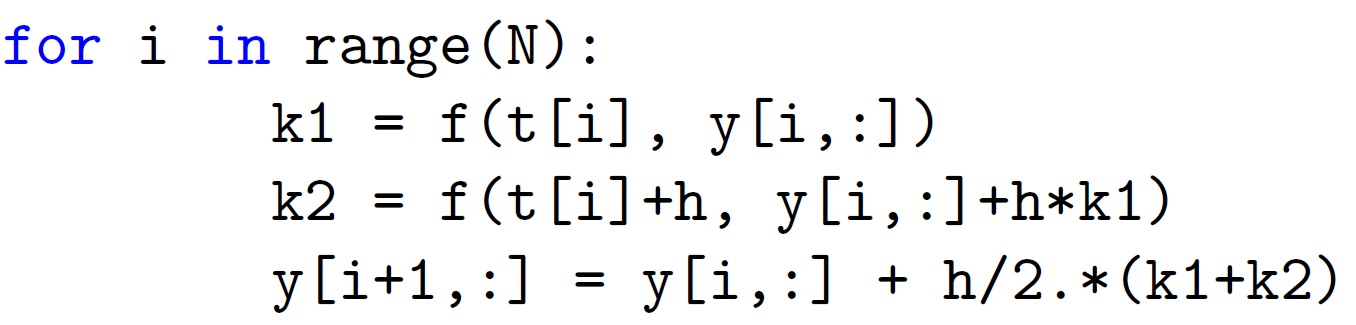
\includegraphics[width=0.25\textwidth]{Figures/RK_eT.png}
\end{center}

$\vec{k}_1 := \vec{f}(t_0 , \vec{y} (t_0))$ und
$\vec{k}_2 := \vec{f}(t_0 + h , \vec{y}(t_0) + h \vec{f}(t_0, \vec{y}_0))$,
dann ist $\vec{y}_1 = \vec{y}_0 + \frac{h}{2} (\vec{k}_1 + \vec{k}_2)$

\vspace{1\baselineskip}

\fat{Polygonzugverfahren}: Die drei Polygonzugverfahren sind jeweils $s=1$-stufige RK
Verfahren.

\vspace{1\baselineskip}

\fat{s-stufiges RK-Verfahren}

Gegeben sind $b_i$ und $a_{ij}$ in $\R$ mit $i,j = 1,\dots,s$ und $\sum_{i=1}^s b_i = 1$.
Dann ist $c_i := \sum_{j=1}^s a_{ij}$ und definiere:

\vspace{1\baselineskip}

\fat{Vorgehen}: (Allgemeines RK-Verfahren)

Berechne: $\vec{k}_i := \vec{f}(t_0 + c_i h , \vec{y}_0 + h \sum_{j=1}^s a_{ij} \vec{k}_j)$
\ \ mit $i=1,\dots,s$

Daraus: $\vec{y}_{j+1} = \vec{y}_j + h \sum:{i=1}^s b_i \vec{k}_i$

\vspace{1\baselineskip}

\Definition{

    Das \fat{Butcher-Tableau} zur Darstellung eines RK-Verfahrens:

    \begin{center}
        \begin{tabular}{c|ccc}
            $c_{1}$ & $a_{11}$ & $\dots$ & $a_{1 s}$ \\
            $\vdots$ & $\vdots$ & & $\vdots$ \\
            $c_{s}$ & $a_{s 1}$ & $\dots$ & $a_{s s}$ \\
            \hline & $b_{1}$ & $\dots$ & $b_{s}$
            \end{tabular} \ \ $=:$ \ \ \begin{tabular}{c|c}
            $\vec{c}$ & $A$ \\
            \hline
            & $(\vec{b})^T$
        \end{tabular}
    \end{center}    
}

Ein RK-Verfahren heisst:
\begin{itemize}
    \item \fat{explizit}, falls $A$ eine strikte untere Dreiecksmatrix ist. Da sich jedes
        $k_i$ aus den früher berechneten $k_i$'s bestimmen lässt, müssen keine inpliziten
        Gleichungen gelöst werden.
    \item \fat{diagonal implizit}, falls $A$ eine nicht-strikte untere Dreiecksmatrix ist.
        Es kann nacheinander eine Gleichung für das neue $k_i$ aufgestellt werden.
    \item \fat{implizit}, sonst. Es muss eine grosse Gleichung mit allen $k_i$'s als
        Unbekannten auf eine Schlange gelöst werden. Dies benötigt den grössten und
        kompliziertesten Rechenaufwand.
\end{itemize}

\vspace{1\baselineskip}

\fat{Beispiele}:

\vspace{1\baselineskip}

eE:
\begin{tabular}{c|c}
    $0$ & $0$ \\
    \hline & $1$
\end{tabular}
\quad
iE: \begin{tabular}{c|c}
    $1$ & $1$ \\
    \hline & $1$
\end{tabular}
\quad
iM: \begin{tabular}{c|c}
    $\frac{1}{2}$ & $\frac{1}{2}$ \\
    \hline & $1$
\end{tabular}

\vspace{1\baselineskip}

eT: \begin{tabular}{c|cc}
    $0$ & $0$ & $0$ \\
    $1$ & $1$ & $0$ \\
    \hline & $\frac{1}{2}$ & $\frac{1}{2}$ 
\end{tabular}
\quad
eM: \begin{tabular}{c|cc}
    $0$ & $0$ & $0$ \\
    $\frac{1}{2}$ & $\frac{1}{2}$ & 0 \\
    \hline & $0$ & $1$
\end{tabular}

\pagebreak

\underline{\fat{Gauss-Kollokation}}

\underline{Motivation}: Nutze Analog zu Gauss-Legendre QF die maximale Ordnung eines
$s$-stufigen RK-Verfahrens aus:
\begin{itemize}
    \item Explizites Verfahren: Ordnung $p \leq s$
    \item Implizites Verfahren: Ordnung $p \leq 2s$
\end{itemize}
\underline{Idee}: Approximiere $y(t)$ zwischen $t_0$ und $t_0 + h$ durch ein
Polynom von Grad $s$ (= Kollokationspolynom $u(t)$), welches die DGL an den Punkten
$t_0 + c_i h \in [t_0 , t_0 + h]$ erfüllt:
\begin{align*}
    \begin{cases}
        u(t_0) = y_0 \\
        \dot{u}(t + c_i h) = f(t_0 + c_i h , u(t_0+c_i h)) \ \
        \forall i \in \geschwungeneklammer{1,\dots,s}
    \end{cases}
\end{align*}
Lösen mit: RK-Verfahren mit $a_{ij} := \int_0^{c_i} l_j (t) dt$,
$b_i := \int_0^1 l_i (t) dt$ mit $l_i(t)$ den Lagrange-Polynomen $\forall i \in
\geschwungeneklammer{1,\dots,n}$ und $c_i$ den Knoten der Gauss-Legendre-QF
(hier: Knoten $\hat{=}$ NST des $s$-ten verschobenen Legendre Polynomes
$P_s (x) := \frac{ds}{dx^s} (x^s (x-1)^s)$)

\vspace{1\baselineskip}

\underline{Konkret}:
Kollokationsverfahren sind implizite RK-Verfahren mit speziellen Einträgen im
Butcher-Tableau.

\vspace{1\baselineskip}

\Beispiel{ (Gauss-Koll. zu $s=2$)

\vspace{1\baselineskip}

    \begin{tabular}{c|cc}
        $\frac{1}{2} - \frac{\sqrt{3}}{6}$ & $\frac{1}{4}$ & $\frac{1}{2} - \frac{\sqrt{3}}{6}$ \\
        $\frac{1}{2} + \frac{\sqrt{3}}{6}$ & $\frac{1}{4} + \frac{\sqrt{3}}{6}$ & $\frac{1}{4}$ \\
        \hline & $\frac{1}{2}$ & $\frac{1}{2}$
    \end{tabular}

    Knoten $c_{1,2} = \frac{1}{2} \pm \frac{\sqrt{3}}{6}$
}

\vspace{1\baselineskip}

\underline{\fat{Adaptivität/ Partitioniertes RK}}

Bisher: Schrittweite $h$= konst.

\underline{Idee}: Verkleinere $h$, wo $f$ schwierig, vergrössere $h$ wo $f$ einfach.

\underline{Vorgehen}: Verwende zwei RK-Verfahren unterschiedlicher Ordnung
(Code: $\Psi_{\text{high}}$, $\Psi_{\text{low}}$) und berechne den lokalen Fehler.
$\Rightarrow$
\begin{itemize}
    \item lok. Fehler gross: $h_{\text{neu}} := \frac{h}{2}$
    \item lok. Fehler klein: $h_{\text{neu}} := c \cdot h$ ($c > 1)$ zB. $1.1$
\end{itemize}

\underline{Wichtig!}: rhs mus formell Zeitabhängig sein!


\vspace{1\baselineskip}

\section{Steife DGL}

\vspace{1\baselineskip}

\Definition{

    Eine DGL ist steif, falls shc das Verhalten der numerischen Lösungen eines expliziten
    Verfahrens ab einem bestimmten $N$ bzw. $h$ komplett verändert.
}

\vspace{1\baselineskip}

\fat{Vorgehen}
(Wie zeigt man dass eine DGL steif ist?)

Wir müssen zeigen, dass sich ab einem $h$ bzw. $N$ das Verhalten komplett ändert:
\begin{itemize}
    \item \fat{Analytisch}: Direkt die Definition eines expliziten Verfahrens
        (am einfachsten eE) verwenden und dies soweit umformen, bis man eine
        Fallunterscheidung des Konvergenzverhaltens in Abhängigkeit von $h$ hat.
    \item \fat{Numerisch}: Man implementiert ein beliebiges explizites Verfahren
        (am besten eM, eE geht auch) und probiert verschiedene $N$, bzw $h$ aus.
        (zB. $10$ bis $10^6$)
\end{itemize}

\vspace{1\baselineskip}

\underline{\fat{Stabilitätsbegriffe}}

\vspace{1\baselineskip}

\fat{Testgleichung}

Die eindimensionale DGL $\dot{y} = \lambda y =: f(y)$ mit $\lambda \in \R$ oder
$\lambda \in \C$ heisst die \fat{Testgleichung}. Damit definieren wir:

\vspace{1\baselineskip}

\fat{Stabilitätsfunktion}

Die Funktion $S: D \subset \C \rightarrow \C$ heisst \fat{Stabilitätsfunktion} eines
Verfahrens, falls für einen Zeitschritt des Verfahrens angewandt auf die Testgleichung
$\dot{y} = \lambda y$ gilt: $y_{k+1} = S(z) y_k$ mit $z := \lambda \cdot h$.

\vspace{1\baselineskip}

\fat{Stabilitätsgebiet}

$S_{\Psi} := \geschwungeneklammer{z \in D \ | \ \abs{S(z)} < 1} \subset \C$

\vspace{1\baselineskip}

\Bemerkung{

    Für ein $s$-stufiges RK-Ein-Schritt-Verfahren mit Butcher-Tableau
    \begin{tabular}{c|c}
        $\vec{c}$ & $A$ \\
        \hline & $(\vec{b})^T$
    \end{tabular}
    gilt:
    $S(z) = \frac{\det \klammer{E_n - z A + z \vec{1} \cdot (\vec{b})^T}}{\det \klammer{E_n - z A}}$
    wobei $\vec{1} = (1,\dots,1)^T \in \R^n$
}

\vspace{1\baselineskip}

\fat{Vorgehen}
(Allgemeine Berechnung)

Bei RK-Verfahren: $S(z)$ mit Formel, sonst:

- Schreibe Def. des Verfahrens $y_{k+1} = F(\text{Verfahren},y_k)$ auf

- Setze für $f(y)$ überall $\lambda y$ ein

Forme so lange um, bis man die Formel $y_{k+1} = S(\lambda h) y_k = S(z) y_k$ erreicht hat

Berechnung von $S_{\Psi}$ direkt mit Definition $\abs{S(z)} < 1$

\vspace{1\baselineskip}

\Definition{

    Ein Verfahren heisst \fat{A-stabil}, falls die (ganze) linke komplexe Ebene im
    Stabilitätsgebiet des Verfahrens ist. $\C^- \subset S_{\Psi}$
}

\vspace{1\baselineskip}

\Definition{

    Ein Verfahren heisst \fat{L-stabil}, falls sie A-stabil ist und
    $S(-\infty) = \limes{z \rightarrow - \infty} S(z) = 0$
}

\vspace{1\baselineskip}

\underline{\fat{Radau Verfahren}}

\vspace{1\baselineskip}

\fat{ROW2} (Ordnung 2)

In jedem Schritt: Berechne $k_1 , k_2$ welche durch diese lineare Gleichungen definiert sind:
\begin{align*}
    (E_n - a h J) \vec{k}_1 &= \vec{f} (\vec{y}_i) \\
    (E_n - a h J) \vec{k}_2 &= \vec{f} (\vec{y}_i + \frac{h}{2} \vec{k}_1) - a h J \vec{k}_1 \\
    \vec{y}_{i+1} &= \vec{y}_i + h \vec{k}_2
\end{align*}
mit $a = \frac{1}{2 + \sqrt{2}}$ und $J = Df(\vec{y_i})$ die Jacobi-Matrix von $f$ an der
letzten Stelle.

\vspace{1\baselineskip}

\fat{ROW3} (Ordnung 3)

Analog mit drei linearen GLS:
\begin{align*}
    (E_n - a h J) \vec{k}_1 &= \vec{f} (\vec{y}_i) \\
    (E_n - a h J) \vec{k}_2 &= \vec{f} (\vec{y}_i + \frac{h}{2} \vec{k}_1) - a h J \vec{k}_1 \\
    (E_n - a h J) \vec{k}_3 &= \vec{f} (\vec{y}_i + h \vec{k}_2) - d_{31} h J \vec{k}_1 - d_{32} h J \vec{k}_2 \\
    \vec{y}_{i+1} &= \vec{y}_i + \frac{h}{6} \klammer{\vec{k}_1 + 4 \vec{k}_2 + \vec{k}_3}
\end{align*}
mit $a = \frac{1}{2 + \sqrt{2}}$, $d_{31} = - \frac{4+ \sqrt{2}}{2 + \sqrt{2}}$,
$d_{32} = \frac{6+ \sqrt{2}}{2 + \sqrt{2}}$ und $J = Df(\vec{y_i})$


\vspace{1\baselineskip}

\section{Nullstellensuche}

\vspace{1\baselineskip}

Geg.: $F: U \subset \R^n \rightarrow \R^n$ eine beliebige Funktion

Ges.: $x^{\star} \in \R^n$ s.d. $F(x^{\star}) = 0$

\vspace{1\baselineskip}

\Definition{ (Iteratives Verfahren)

    Ein Iteratives Verfahren ist ein Algorithmus definiert durch:

    - Einen Startwert $x_0$

    - Eine Iterationsvorschrift $x_{k+1} = \phi (x_k)$

    - Eine Abbruchbedingung, wie zB.

        \hspace{10pt} - Max. Anzahl Schritte

        \hspace{10pt} - Absolute Toleranz: $\Norm{x_{k+1} - x_k} <$ abstol

        \hspace{10pt} - Relative Toleranz: $\frac{\Norm{x_{k+1} - x_k}}{\Norm{x_{k+1}}} <$ reltol

    Somit erzeugt es eine Folge $x_1 , \dots , x_N$ von approximierten Lösungen zu einem
    Problem.
}

\vspace{1\baselineskip}

\Definition{

    Sei $\limes{k \rightarrow \infty} x_k = x^\star$ für ein $x^\star$.
    Dann ist der \fat{Fehler} definiert als: $e_k := \Norm{x^\star - x_k}$.
    In der Regel ist $x^\star$ nicht bekannt. Dann: $x^\star \approx x_N$ für
    $N>>1$, $e_k \approx \Norm{x_N - x_k}$.
}

\vspace{1\baselineskip}

\Definition{ (Konvergenzordnung $p$)

    Sei $c>0$ sodass $e_{k+1} \leq c e_k^p$. Dann folgt die Berechnung:
    \begin{align*}
        \begin{rcases}
            e_{k+1} \approx c e_{k}^p \\
            e_k \approx c e_{k-1}^p
        \end{rcases}
        \Rightarrow
        p \approx \frac{\log \klammer{\frac{e_{k+1}}{e_k}}}{\log \klammer{\frac{e_k}{e_{k-1}}}}
        =: p_k
    \end{align*}
    \underline{Achtung}! $p$ ist ein Array mit einträgen $[p_1,\dots,p_{N-2}]$.
    Wähle für $p$ einfach den letzten "vernünftigen" Eintrag.

    \vspace{1\baselineskip}

    \underline{Wichtig}! Dies ist nicht die selbe Konvergenzordnung wie bei DGL oder
    Quadratur.
}

\vspace{1\baselineskip}

\Definition{

    $x^{(k+1)} = \Phi (x^{\star})$ heisst \fat{linear konvergent} nach $x^\star$, falls
    es ein $L < 1$ gibt, sodass:
    \begin{align*}
        \Norm{x^{(k+1)} - x^{\star}} \leq L \Norm{x^{(k)} - x^\star}
        \ \ \ \forall k \in \N
    \end{align*}
}

\vspace{1\baselineskip}

\Bemerkung{
    \begin{align*}
        \Norm{x^{(k+1)} - x^{\star}} \leq L \Norm{x^{(k)} - x^\star} \leq L^{k+1} \Norm{x^{(0)} - x^\star}
    \end{align*}
}

\vspace{1\baselineskip}

\Definition{

    \fat{Konvergenzordnung $p$} des Iterativen Verfahrens heisst, es gibt ein $C>0$, sodass
    \begin{align*}
        \Norm{x^{(k+1)} - x^\star} \leq C \cdot \Norm{x^{(k)} - x^\star}^p
    \end{align*}
}

\vspace{1\baselineskip}

\Bemerkung{

    Bei linearer Konvergenz und bekanntem $L$ kann man folgende Abschätzung machen:
    \begin{align*}
        \Norm{x^{(k+1)} - x^\star} \leq \frac{1}{1-L} \Norm{x^{(k+1)} - x^{(k)}}
    \end{align*}
}

\pagebreak

\underline{\fat{Fixpunktiteration}}

\vspace{1\baselineskip}

\fat{Vorgehen}

Wähle ein $\phi(x)$. Iteratives Verfahren mit Iterationsvorschrift:
$x_{k+1} = \phi (x)$

\vspace{1\baselineskip}

\fat{Konvergenz}

\vspace{1\baselineskip}

\Definition{

    Eine Funktion $\phi$ heisst \fat{Kontraktion}, falls es ein $L>1$ gibt, so dass
    $\Norm{\phi(x) - \phi(y)} \leq L \Norm{x-y}$ für alle $x,y$.
}

\vspace{1\baselineskip}

\Bemerkung{

    Wenn $x^\star$ ein Fixpunkt der Kontraktion $\phi$ ist, dann ist
    \begin{align*}
        \Norm{x^{(k+1)} - x^\star} = \Norm{\phi (x^{(k)}) - \phi(x^\star)}
        \leq L \Norm{x^{(k)} - x^\star}
    \end{align*}
    Das heisst, dass das iterative Verfahren $x^{k+1} = \phi (x^k)$ mindestens linear
    konvergiert.
}

\vspace{1\baselineskip}

\Satz{

    Sei $D \subset \K^n$ ($\K = \R , \C$), mit $D$ abgeschlossen, und $\phi:D \rightarrow D$
    einer Kontraktion. Dann existiert ein eindeutiger Fixpunkt $x^\star$, also
    $\phi(x^\star) = x^\star$. Dieser ist der Grenzwert der Folge $x^{(k+1)} = \phi(x^{(k)})$.
}

\vspace{1\baselineskip}

\Satz{ (Hinreichende Bedingung für lokale lineare Konvergenz einer Fixpunktiteration)

    Es Sei $U$ konvex und $\phi:U \subset \R^n \rightarrow \R^n$ stetig differenzierbar
    mit $L := \sup_{x \in U} \Norm{D \phi(x)} < 1$ wobei ($D \phi (x)$ die Jacobi-Matrix
    von $phi$ ist). Wenn $\phi(x^\star) = x^\star$ für $x^\star \in U$, dann konvergiert
    die Fixpunktiteration $x^{(k+1)} = \phi(x^{(k)})$ gegen $x^\star$ lokal mindestens
    linear.
}

\vspace{1\baselineskip}

\Satz{

    Sei $\phi: \R^n \rightarrow \R^n$ mit $\phi(x^\star) = x^\star$ und $\phi$ stetig
    differenzierbar in $x^\star$. Ist $\Norm{D\phi(x^\star)} < 1$, dann konvergiert die
    Fixpunktiteration $x^{(k+1)} = \phi (x^{(k)})$ lokal (mindestens) linear, mit
    $L = \Norm{D \phi (x^\star)}$.
}

\vspace{1\baselineskip}

\Satz{

    Sei $U \subset \R$ ein Intervall und $\phi: U \rightarrow \R$ $(m+1)$-mal differenzierbar
    mit $\phi(x^\star) = x^\star \in U$. Sei weiterhin $\phi^{(l)} (x^{\star}) = 0$ für
    $l=1,\dots,m$ ($m \geq 1$). Dann konvergiert die Fixpunktiteration
    $x^{(k+1)} = \phi(x^{(k)})$ gegen $x^\star$ lokal der Ordnung $p \geq m+1$.
}

\vspace{1\baselineskip}

\Lemma{

    Konvergiert die Kontraktion $\phi$ linear mit dem Faktor $L<1$, dann gilt die
    folgende Abschätzung:
    \begin{align*}
        \Norm{x^\star - x^{(k)}} \leq \frac{L^{k-l}}{1-L} \Norm{x^{(l+1)} - x^{(l)}}
    \end{align*}
}

\vspace{1\baselineskip}

\underline{\fat{Bisektionsverfahren (Intervallhalbierungsverfahren)}}

\vspace{1\baselineskip}

\underline{Idee}: Zwischenwertsatz:
$F:[a,b] \rightarrow \R$ stetig mit $F(a) F(b) < 0 \Rightarrow \exists x^\star \in [a,b]$
sodass $F(x^\star) = 0$

\underline{Vorgehen}:
Iteratives Verfahren mit der Iterationsvorschrift:

- Intervall halbieren $m=\frac{a+b}{2}$

- Suche Intervall mit unterschiedlichen Vorzeichen:
$F(a) F(m) < 0$ oder $F(m) F(b) < 0$

- Weiter mit Intervall "$<0$"

\vspace{1\baselineskip}

Konvergiert immer. Lineare Konvergenz. Keine verallgemeinerung in mehreren
Dimensionen.

\vspace{1\baselineskip}

\underline{\fat{Newtonverfahren}}

\vspace{1\baselineskip}

\underline{Idee}
Approximation von $F$ durch Tangente bei $x_k$ (Taylor):

$F(x) \approx \tilde{F} (x) := F(x_k) + F'(x) \cdot (x-x_k) \stackrel{!}{=} 0$

\underline{Vorgehen}:
(Newtonverfahren)

Iteratives Verfahren mit Iterationsvorschrift:
$x_{k+1} = x_k - \frac{F(x_k)}{F'(x_k)}$

\vspace{1\baselineskip}

\underline{Mehrdimensional}

Gleiche Idee: $x_{k+1} = x_k - DF(x_k)^{-1} F(x_k) := x_k - s_k$
Aber $DF(x_k) := (\frac{\partial F_i}{\partial x_j})_{ij} \in \Mat(n \times n;\R)$
"Berechne nie das Inverse einer Matrix!"

\underline{Vorgehen}
(Mehrdimensionales Newtonverfahren)

Iteratives Verfahren mit Iterationsvorschrift:

- $\vec{s}_k =$ Lösung des linearen GLS $DF(\vec{x}_k) \vec{s}_k = F (\vec{x}_k)$

- $\vec{x}_{k+1} = \vec{x}_k - \vec{s}_k$

Newtonverfahren = Fixpunktiteration mit $\phi(x) = x- \frac{F(x)}{F'(x)}$
$\Rightarrow$ lokal mindestens quadratische Konvergenz.

\vspace{1\baselineskip}

\underline{Sekantenverfahren}

Falls $F'$ unbekannt: $F'(x) \approx \frac{F(x_k) - F(x_{k-1})}{x_k - x_{k-1}}$

Konvergenzordnung: $p \approx 1.62$

Beachte: 2. Startwert benötigt. Mehrdimensional nicht möchlich.

\vspace{1\baselineskip}

\underline{\fat{Gedämpftes Newtonverfahren}}

\vspace{1\baselineskip}

\underline{Idee}:
Dämfung von $s_k$ mit einem Dämpfungsparameter $\lambda_k \in (0,1]$

Es wird das maximale $\lambda_k$ gewählt, so dass
\begin{align*}
    \Norm{\frac{F \klammer{x^{(k)} - \lambda^{(k)} \frac{F(x^{(k)})}{DF(x^{(k)})}}}{DF(x^{k})}}_2
    \leq
    \klammer{1-\frac{\lambda^{(k)}}{2}} \Norm{\frac{F(x^{(k)})}{DF(x^{(k)})}}_2
\end{align*}
Praxis: $\lambda_k = 1 \rightarrow \frac{1}{2} \rightarrow \frac{1}{4} \rightarrow \dots$
bis die obere Bedingung erfüllt ist.

\vspace{1\baselineskip}

\underline{Vorgehen}:
(Gedämpftes Newtonverfahren)

Iteratives Verfahren mit Iterationsvorschrift:

- $\vec{s}_k =$ Lösung von $DF(\vec{x}_k) \vec{s}_k = F(\vec{x}_k)$ oder in 1D: $\frac{F(x_k)}{F'(x_k)}$

- $\lambda_k = \max \geschwungeneklammer{\frac{1}{2^n} \ | \ n \in \N_0 \text{ und erfüllt obige Bedingung}}$
(in jedem Iterstionsschritt neu berechnen!)

- $\vec{x}_{k+1} = \vec{x}_k - \lambda_k \vec{s}_k$

\vspace{1\baselineskip}

\underline{\fat{Quasi-Newtonverfahren}}

\vspace{1\baselineskip}

\underline{Broyden Verfahren}

Setze $J_0 = DF(x_0) \in M(n \times n , \R)$ und löse für $k=1,2,\dots$
\begin{align*}
    \begin{cases}
        J_k \cdot s_k = F(x_k) \ \Leftrightarrow s_k = \text{solve} (J_k , F(x_k))
        \\
        x_{k+1} = x_k - s_k
        \\
        J_{k+1} = J_k + \frac{1}{\Norm{s_k}^2} F(x_{k+1}) (-s_k)^T
    \end{cases}
\end{align*}

\vspace{1\baselineskip}

\underline{Sherman-Morrison-Formel}
\begin{align*}
    J_{k+1}^{-1} = J_k^{-1} + \frac{J_k^{-1} F(x_{k+1}) s_k^T J_k^{-1}}{\Norm{s_k}^2 - s_k^T J_k^{-1} F(x_{k+1})}
\end{align*}

\vspace{1\baselineskip}

Daraus entsteht folgende \underline{Iteration}:
\begin{enumerate}
    \item Schritt:
        \begin{align*}
            \begin{cases}
                J_0 = DF(x_0) \\
                s_0 = \text{solve} (J_0 , F(x_0)) \\
                x_1 = x_0 - s_0
            \end{cases}
        \end{align*}
    \item Schritt:
        \begin{align*}
            \begin{cases}
                J_1^{-1} = J_0^{-1} + \frac{J_0^{-1} F(x_{1}) s_0^T J_0^{-1}}{\Norm{s_0}^2 - s_0^T J_0^{-1} F(x_{1})}
                \\
                s_1 = J_1^{-1} F(x_1)
                \\
                x_2 = x_1 - s_1
                \\
                \vdots
            \end{cases}
        \end{align*}
\end{enumerate}

\underline{Alternativ}
\begin{align*}
    s_{k+1} = J_{k+1}^{-1} F(x_{k+1})= J_{k}^{-1} F(x_{k+1}) + \frac{J_k^{-1} F(x_{k+1}) s_k^T J_k^{-1} F(x_{k+1})}{\Norm{s_k}^2 - s_k^T J_k^{-1} F(x_{k+1})}
\end{align*}
Wir definieren nun $w_k := J_{k}^{-1} F(k+1)$ (Lsg. des GLS $J_k w_k = F(x_{k+1})$)
und $z_k := s_k^T w_k$.
Dann folgt:
\begin{align*}
    S_{k+1} = \klammer{1 + \frac{z_k}{\Norm{s_k}^2 - z_k}} w_k
\end{align*}



\vspace{1\baselineskip}

\section{Numerische Lineare Algebra}

\vspace{1\baselineskip}

\Bemerkung{

\vspace{1\baselineskip}

\footnotesize

    \begin{tabular}{c|c}
        \fat{Invertierbar} & \fat{Nicht invertierbar} \\
        \hline $A$ ist regulär & $A$ ist singulär \\
        Zeilen sind linear unabhängig & Zeile sind linear abhängig \\
        Spalten sind linear unabhängig & Spalten sind linear abhängig \\
        $\det A \neq 0$ & $\det A = 0$ \\
        $A x = 0$ hat eine Lösung $x=0$ & $Ax=0$ hat $\infty$ viele Lösungen \\
        $Ax=b$ hat eine Lösung $x = A^{-1} b$ & $Ax=b$ hat keine oder $\infty$ Lösungen \\
        $A$ hat vollen Rang & $A$ hat Rang $r<n$ \\
        $A$ hat $n$-nicht-Null-Pivoten & $A$ hat $r<n$ Pivoten \\
        $\text{span} \geschwungeneklammer{A_{:,1} , \dots , A_{:,n}}$ hat dim $n$ &
        $\text{span} \geschwungeneklammer{A_{:,1},\dots,A_{:,n}}$ hat dim $r<n$ \\
        $\text{span} \geschwungeneklammer{A_{1,:} , \dots , A_{n,:}}$ hat dim $n$ &
        $\text{span} \geschwungeneklammer{A_{1,:},\dots,A_{n,:}}$ hat dim $r<n$ \\
        Alle Eigenwerte von $A$ sind $\neq 0$ & $0$ ist EW von $A$ \\
        $0 \notin \sigma(A) =$ Spektrum von $A$ & $0 \in \sigma (A)$ \\
        $A^H A$ ist symmetrisch positiv definit & $A^H A$ ist semidefinit \\
        $A$ hat $n$ (positive) Singulärwerte & $A$ hat $r<n$ (positive) Singulärwerte
    \end{tabular}
\normalsize
}

\vspace{1\baselineskip}

\Bemerkung{

    Orthogonale/Unitäre Transformationen erhalten die euklidische Norm:
    \begin{align*}
        \Norm{Qx}_2^2 = (Q x)^H (Q_x) = x^H Q^H Q x = x^H E_n x = \Norm{x}_2^2
    \end{align*}
}

\vspace{1\baselineskip}

\underline{\fat{LU-Zerlegung}}

Sei $A \in \R^{n \times n}$ invertierbar, dann existieren $P,L,U \in \R^{n \times n}$, so
dass $PA = LU$. Wobei $L$ eine untere Dreiecksmatrix mit einsen auf der Diagonalen,
$U$ eine obere Dreiecksmatrix und $P$ eine Permutationsmatrix sind.

Anwendung: Lösen von GLS

$Ax = b \Leftrightarrow LU x = Pb \Leftrightarrow Lz = Pb$ (Vorwärtssubstitution) und
$U x = z$ (Rückwärtssubstitution)

Code: P,L,U = scipy.linalg.lu(A)

\pagebreak

\underline{\fat{Cholesky-Zerlegung}}

Ist $A$ symetrisch $(a=A^T)$ und positiv definit, dann existiert eine Zerlegung
$A=LL^T = U^T U$, wobei $L$ und $U$ untere Dreiecksmatrizen sind mit strikt positiven
Diagonaleinträgen.

Anwendung: $A=LL^T  \Rightarrow Ax = LL^T x = b \Leftrightarrow L y = b \Rightarrow$
    finde $y \Rightarrow L^T x = y \Rightarrow$ finde $x$.

Code: L = numpy.linalg.cholesky(A)

\vspace{1\baselineskip}

\underline{\fat{QR-Zerlegung}}

Sei $A \in \R^{m \times n}$ mit $m \geq n$, dann existiert ein $\hat{Q} \in \R^{m \times n}$,
und ein $\hat{R} \in \R^{n \times n}$, so dass $A = \hat{Q} \hat{R}$ wobei $\hat{Q}$
orthogonale Spalten hat und $\hat{R}$ eine obere Dreiecksmatrix ist.
(reduzierte $QR$-Zerlegung)

Bem: $A = QR$, wobei $Q := (\hat{Q} \ q_{n+1} \ \dots \ q_m) \in \R^{m \times m}$ und
$R:= (\hat{R} \ 0)^T \in \R^{m \times n}$. Mit $Q^T Q = E_m$ (orthogonal)
(vollständige $QR$-Zerlegung)

Code: Qhat, Rhat = numpy.linalg.qr(A) \ \ \ \ oder 

\hspace{27pt} Q,R = numpy.linalg.qr(A,mode='complete')

\vspace{1\baselineskip}

\underline{Methoden}:

\vspace{1\baselineskip}

\fat{Gram-Schmidt-Verfahren}

Orthogonalisiere die Spalten von $A$ $\Rightarrow Q$.
Finde danach $R$, sodass gilt: $QR=A$.

\vspace{1\baselineskip}

QR via \fat{Rotation}:
\footnotesize
\begin{align*}
    G_{ij} (\varphi) = 
    \eckigeklammer{
    \begin{array}{*{11}c}
        1 & & & & & & & & & & \\
        & \dots & & & & & & & & & \\
        & & 1 & & & & & & & & \\
        & & & \cos(\varphi) & & & & \sin(\varphi) & & & \\
        & & & & 1 & & & & & & \\
        & & & & & \ddots & & & & & \\
        & & & & & & 1 & & & & \\
        & & & - \sin(\varphi) & & & & \cos(\varphi) & & & \\ 
        & & & & & & & & 1 & & \\
        & & & & & & & & & \ddots & \\
        & & & & & & & & & & 1
    \end{array} 
    }
\end{align*}
\normalsize
mit $\cos(\varphi)$ an der $ii$-ten und $jj$-ten Stelle. Und $\sin(\varphi)$ an der
$ij$-ten Stelle, sowie $- \sin(\varphi)$ an der $ji$-ten Stelle.
Dabei gilt:
\begin{align*}
    r = \sqrt{x_i^2 + x_j^2}
    \quad
    \cos(\varphi) = \frac{x_i}{r}
    \quad
    \sin(\varphi) = \frac{x_j}{r}
\end{align*}
Dann folgt:
\begin{align*}
    G_{ij} (\varphi) \cdot \begin{bmatrix}
        x_i \\ \cdots \\ x_{i-1} \\ x_i \\ x_{i+1} \\ \vdots \\ x_{j-1} \\ x_j \\ x_{j+1}
        \\ \vdots \\ x_n
    \end{bmatrix}
    =
    \begin{bmatrix}
        x_i \\ \cdots \\ x_{i-1} \\ r \\ x_{i+1} \\ \vdots \\ x_{j-1} \\ 0 \\ x_{j+1}
        \\ \vdots \\ x_n
    \end{bmatrix}
\end{align*}
Mit diesem Verfahren erhält man einen Algorithmus zur Bestimmung von $Q$.

\pagebreak

\fat{Housholder-Spiegelung}

Sei $a$ der Startvektor := erste Spalte von $A$. Dann folgt der folgende Algorithmus:
\begin{align*}
    &v := \begin{cases}
        \frac{1}{2} \klammer{a + \Norm{a}_2 e_1} \quad \text{ falls } a_1 >0 \ \ (\text{der erste Eintrag von } a)
        \\
        \frac{1}{2} \klammer{a - \Norm{a}_2 e_1} \quad \text{ falls } a_1 < 0
    \end{cases}
    \\
    \\
    &u := \frac{v}{\Norm{v}_2}
    \\
    \\
    &Q^T := E_m - 2 u u^T
\end{align*}
Dies wiederholt man für alle Spalten von $A$. Dann erhält man:
$Q = \klammer{Q_m^T \dots Q_1^T}^T = \klammer{\prod_{i=0}^{m-1} Q_{m-i}^T}^T$

Am Schluss muss man noch $R$ herausfinden:
$R = \klammer{\prod_{i=}^{m} Q_{i}^T} \cdot A$

\vspace{1\baselineskip}

\underline{\fat{Singulärwertzerlegung}}

Sei $A \in \C^{m \times m}$ beliebig. Dann gibt es unitäre Matrizen $V \in \C^{m \times m}$
und $U \in \C^{n \times n}$ und die $m \times n$ Diagonalmatrix in $\sigma = \text{diag}
(\sigma_1 , \dots , \sigma_p)$ mit $p= \min \geschwungeneklammer{m,n}$ und
$\sigma_1 \geq \dots \sigma_p \geq 0$, sodass
\begin{align*}
    A = U \Sigma V^H
\end{align*}

\underline{$m=n \ \Rightarrow \ \Sigma$ ist invertierbar}:

$\Rightarrow Ax=b \Leftrightarrow U \Sigma V^T x = b \Leftrightarrow x = \klammer{U \Sigma V^T}^{-1} b
\Leftrightarrow x = V \Sigma^{-1} U^T b$

Code:

U,s,Vt = scipy.linalg.svd(A)

Sigma.inv = np.diag(1/s)

x = np.dot(Vt.T , np.dot(Sigma.inv , np.dot(U.T , y)))

\vspace{1\baselineskip}

\underline{$m \neq n \ \Rightarrow \ \rang(\Sigma) = r < p = \min \geschwungeneklammer{m,n}$}:
(reduzierte SVD)
\begin{enumerate}
    \item Zerlege $A = U \Sigma V^T =$
        \begin{align*}
            A=
            \begin{pmatrix} U_1 &  U_2 \end{pmatrix}
            \begin{pmatrix}
                \Sigma_r & \\ 0 & 0
            \end{pmatrix}
            \begin{pmatrix}
                V_1^T \\ V_2^T
            \end{pmatrix}
        \end{align*}
        mit $U_1 \in M(m \times r ; K), \ \Sigma_r \in M(r \times r; K), \ V_1^T \in M(r \times n ; K),
        \ A \in M(m \times n;K)$, dann ist $\Sigma_r^{-1}$ wohldefiniert und ist gegeben durch:
        \begin{align*}
            \Sigma_r^{-1} = \begin{pmatrix}
                \frac{1}{\sigma_1} & & \\
                & \dots & \\
                & & \frac{1}{\sigma_r}
            \end{pmatrix}
        \end{align*}
    \item Schreibe um: $Ax=b \Leftrightarrow U_1 \Sigma_r V_1^T x = b \Leftrightarrow
        x = V_1 \Sigma_r^{-1} U_1^T b$. Man nenne $V_1 \Sigma_r^{-1} U_1^T$ auch die
        \fat{Pseudoinverse} von $A$.
\end{enumerate}

\vspace{1\baselineskip}

\underline{\fat{Kondition}}

\vspace{1\baselineskip}

\Definition{

    Die \fat{Konditionszahl} einer Matrix $A$ ist cond$(A) := \Norm{A^{-1}} \cdot \Norm{A}$
}

\vspace{1\baselineskip}

\Definition{

    Die \fat{Matrixnorm} ist gegeben als:
    \begin{align*}
        \Norm{A} := \sup_{\Norm{x} \neq 0} \frac{\Norm{Ax}}{\Norm{x}} =
            \sup_{\Norm{x}=1} \Norm{Ax}
    \end{align*}
}

\pagebreak

\Theorem{

    Wenn die Singulärwerte von $A$ erfüllen:
    \begin{align*}
        \sigma_1 \geq \sigma_2 \geq \dots \geq \Sigma_r > \sigma_{r+1} = \sigma_p = 0
    \end{align*}
    dann gilt: $\rang A = r$ und:
    \begin{align*}
        \ker A &= \text{span} \geschwungeneklammer{v_{r+1} , \dots , v_n} \\
        \Im A &= \text{span} \geschwungeneklammer{u_1,\dots,u_r}
    \end{align*}
}

\vspace{1\baselineskip}

\Bemerkung{

    Gegeben $A \in \C^{m \times n}$ mit $m>n$, finde $x \in \C^n$ mit $\Norm{x}=1$,
    sodass $\Norm{Ax}_2$ minimal wird. Die SVD hilft, denn unitäre Matrizen erhalten die
    $2$-Norm:
    \begin{align*}
        \min_{\Norm{x}=1} \Norm{Ax}_{2}^2 &= \min_{\Norm{x}=1} \Norm{U \Sigma V_x^H}_2^2
        = \min_{\Norm{V_x^H}_2=1} = \min_{\Norm{y}_2 = 1} \Norm{\Sigma y}_2^2
        \\
        &= \min_{\Norm{y}_2 = 1} (\sigma_1^2 y_1^2 + \dots + \sigma_n^2 y_n^2)
        \geq \sigma_n^2
    \end{align*}
}

\vspace{1\baselineskip}

\Theorem{

    Sei $A \in \C^n$. Dann gilt: $\Norm{A}_2 = \sigma_1 (A)$. Falls $A$ invertierbar ist,
    dann gilt:
    \begin{align*}
        \text{cond}_2 (A) = \frac{\sigma_1}{\sigma_m}
    \end{align*}
}

\vspace{1\baselineskip}

\Definition{

    Die \fat{Frobeniusnorm} der $m \times n$-Matrix $A$ ist
    \begin{align*}
        \Norm{A}_F^2 := \sum_{i=1}^{m} \sum_{j=1}^n \abs{a_{ij}}^2
    \end{align*}
}

\vspace{1\baselineskip}

\Theorem{

    Für die $m \times n$-Matrix $A$ mit Rang $r$ gelten die Singulärwertzerlegung
    $A = U \Sigma V^H$ mit $m \geq n$ und $U = [\vec{u}_1 \ \dots \ u_{m}]$ und
    $V = [v_1 \ \dots \ v_n]$. Für $k \in \geschwungeneklammer{1,\dots,r}$ sei die
    $m \times k$-Matrix $U_k = [\vec{u}_1 \ \dots \ \vec{u}_k]$, die $n \times k$-Matrix
    $V_k = [\vec{v}_1,\dots,\vec{v}_k]$ und die $k \times k$-Matrix $\Sigma_k :=
    \text{diag} (\sigma_1,\dots,\sigma_k)$. Für $\standardNorm = \standardNorm_F$ und
    $\standardNorm = \standardNorm_2$ gilt dann:
    \begin{align*}
        \Norm{A - U_k \Sigma_k V_k^H} \leq \Norm{A - B}
    \end{align*}
    für alle $m \times n$-Matrizen $B$ von Rang $k$
}


\vspace{1\baselineskip}

\section{Ausgleichsrechnung}

\Bemerkung{

    cond$(A^T A) =$ cond$(A^2)$
}

\vspace{1\baselineskip}

\Bemerkung{

    Norm minimieren: finde $x$ sodass $A^T A x = A^T b$
}

\vspace{1\baselineskip}

\fat{Ausgleichsrechnung}

Geg.: Daten $(t_i,y_i) \in \R^2$, $i \in \geschwungeneklammer{1,\dots,m}$, Modell
$f_{\vec{x}}: \R \rightarrow \R$, $f_{\vec{x}} (t) = \vec{y}$

Ges. Parameter $\vec{x} = (x_1,\dots,x_n)$, so dass die Daten und das Modell am besten passen.
\begin{align*}
    \text{Wir wollen}:
    \begin{pmatrix}
        f_{\vec{x}} (t_1) \\ \vdots \\ f_{\vec{x}} (t_m)
    \end{pmatrix} = \begin{pmatrix}
        y_1 \\ \vdots \\ y_m
    \end{pmatrix} \Leftrightarrow
    \underbrace{
    \begin{pmatrix}
        \abs{f_{\vec{x}} (t_1) - y_1} \\ \vdots \\ \abs{f_{\vec{x}} (t_m) - y_m}
    \end{pmatrix}
    }_{:=\vec{R} = \text{Residuum / Residuenvektor}}
    = \vec{0}
\end{align*}
Bei der Ausgleichsrechnung: $m > n$. Das erste GLS ist somit überbestimmt und es gibt keine
Lösung. Stattdessen erhalten wir das Minimierungsproblem:

\fat{Least Squares Problem}: $\vec{x^\star} = \text{argmin}_{\vec{x}} \sum_{i=1}^{m}
    \abs{f_{\vec{x}} (t_i) - y_i}^2 = \text{argmin}_{\vec{x}} \Norm{\vec{R}}_2^2$

\vspace{1\baselineskip}

\underline{\fat{Lineare Ausgleichsrechnung}}

Falls $f_{\vec{x}}$ linear im Parameter $\vec{x}$, also $f_{\vec{x}} (t) = x_1 b_1 (t) +
\dots + x_n b_n (t)$ für Basisfunktionen $b_j(t)$ (nicht notwendigerweise linear in $t$),
dann handelt es sich um \fat{lineare Ausgleichsrechnung}. Für diesen Spezialfall lässt sich
das Problem umschreiben zu:
\begin{align*}
    \underbrace{\begin{pmatrix}
        b_1(t_1) & \dots & b_n(t_1) \\
        \vdots& \ddots & \vdots \\
        b_1(t_m) & \dots & b_n(t_n)
    \end{pmatrix}}_{:= A \in M(m \times n;K)}
    \underbrace{\begin{pmatrix}
        x_1 \\ \vdots \\ x_n
    \end{pmatrix}}_{:= \vec{x}}
    = \underbrace{\begin{pmatrix}
        y_1 \\ \vdots \\ x_m
    \end{pmatrix}}_{:= \vec{b}}
    \Leftrightarrow
    A \vec{x} = \vec{b}
    \Leftrightarrow
    \Norm{A \vec{x} - \vec{b}} = 0
\end{align*}
Da $m>n$ ist GLS $A \vec{x} = \vec{b}$ wie im allgemeinen Fall überbestimmt. Wir lösen also
Stattdessen das für den linearen Fall umschriebene \fat{Least Squares Problem}:

$x^\star = \text{argmin}_{\vec{x}} \Norm{A \vec{x} - \vec{b}}_2^2$

Code: numpy.linalg.lstsq(A,b)[0]

\vspace{1\baselineskip}

\underline{Normalengleichung}

Idee: Bestimme Minimum durch: $\grad (\Norm{A \vec{x} - \vec{b}}_2^2) \stackrel{!}{=} 0$

$\vec{x^\star} = \text{argmin} \Norm{A \vec{x} - \vec{b}}_2^2 \Leftrightarrow A^T A \vec{x^\star} = A^T \vec{b}$

Code: ATA = np.dot(A.T,A)

\hspace{27pt} ATb = np.dot(A.T,b)

\hspace{27pt} xstar = numpy.linalg.solve(ATA,ATb)

\vspace{1\baselineskip}

\underline{QR-Zerlegung}

Idee: $A = QR = \hat{Q} \hat{R}$

$\Norm{A \vec{x} - \vec{b}}_2^2 = \Norm{Q R \vec{x} - \vec{b}}_2^2 = \Norm{R \vec{x} - Q^T \vec{b}}_2^2$

$= \Norm{\hat{R} \vec{x} - \hat{Q}^T \vec{b}}_2^2 + \Norm{\begin{pmatrix}
    q_{n+1} \\ \vdots \\ q_m
\end{pmatrix} \vec{b}}_2^2$

Minimiere den von $\vec{x}$ abhängigen Teil exakt:

$\vec{x^\star} = \text{argmin} \Norm{A \vec{x} - \vec{b}}_2^2
\Leftrightarrow \hat{R} \vec{x^\star} = \hat{Q}^T \vec{b}$

Code: Qhat,Rhat = numpy.linalg.qr(A)

\hspace{27pt} xstar = numpy.linalg.solve(Rhat , dot(Qhat.T , b))

\vspace{1\baselineskip}

\underline{Singulärwertzerlegung}

Idee: $A=U \Sigma V^T = \begin{pmatrix} U_1 & | & U_2 \end{pmatrix} \begin{pmatrix}
    \Sigma_r  & 0 \\ 0 & 0 \end{pmatrix} \begin{pmatrix} V_1^T \\ \hline V_2^T \end{pmatrix}$

Dabei ist $r = \rang A =$ Anzahl Singulärwerte $\neq 0$, $u_1 \in \R^{m \times r}$,
$V_1 \in \R^{n \times r}$. Analoge Überlungen wie bei QR liefert:

$\vec{x^\star} = \text{argmin} \Norm{A \vec{x} - \vec{b}}_2^2 \Leftrightarrow \vec{x^\star} =
V_1 \Sigma_r^{-1} U_1^T \vec{b}$

Code: psinvA = numpy.linalg.pinv(A)

\hspace{27pt} xstar = dot(psinvA,b)

\vspace{1\baselineskip}

\underline{Allgemeines Vorgehen}
\begin{enumerate}
    \item Daten implementieren: t = np.array$([t_1,\dots,t_m])$, y = np.array$([y_1,\dots,y_m])$
    \item Basisfunktionen und $A$ bestimmmen:
    
            b = lambda s: np.array$([b_1(s),\dots,b_n(s)])$,
    
            A = np.array$([b(s) \text{ for $s$ in $t$}])$
    \item Ausgleichsrechnung lösen: lstsq, red. QR oder SVD
    \item Lösung plotten:

            tnew = np.linspace(t[0],t[-1],1000)

            f = lambda t : np.dot(x,b(t))

            plt.plot(t,y)

            plt.plot(tnew,f(tnew))
\end{enumerate}

\vspace{1\baselineskip}

\underline{\fat{Nichtlineare-Ausgleichsrechnung}}

$f_{\vec{x}}$ ist nicht linear in $\vec{x}$. Ziel: Minimierung der Quadrate:
$\vec{x^\star} = \text{argmin}_{\vec{x}} \sum_{i=1}^{m} \abs{f_{\vec{x}}(t_i) - y_i}^2$

Definiere:
\begin{align*}
    F(\vec{x}) &:= \begin{pmatrix}
        f_{\vec{x}} (t_1) - y_1 \\ \vdots \\ f_{\vec{x}} (t_m) - y_m
    \end{pmatrix}
    \\
    \phi(\vec{x}) &:= \frac{1}{2} \Norm{F(\vec{x})}_2^2 \rightarrow
    \vec{x^\star} = \text{argmin}_{\vec{x}} \sum_{i=1}^{m} \abs{f_{\vec{x}}(t_i) - y_i}^2
    \\ &\Leftrightarrow \vec{x^\star} = \text{argmin} \phi(\vec{x})
\end{align*}
Code: xstar = scipy.optimize.leastsq$(F,x_0)$[0]

mit $x_0$ einem guten Startwert, oftmals reicht ein Einervektor: x0 = np.ones(n)

\vspace{1\baselineskip}

\underline{Newton Verfahren}

Idee: $\phi(\vec{x})$ minimal $\Leftrightarrow \grad (\phi(\vec{x})) = 0 \Rightarrow$
bestimme NST mit Newtonverfahren. Wir brauchen dazu auch die Ableitung von
$\grad (\phi(\vec{x}))$, also die Hessematrix.

Vorgehen:

- $\grad (\phi(\vec{x})) := (DF( \vec{x}))^T F(\vec{x})$

- $Hess (\phi(\vec{x})) := (DF(\vec{x}))^T DF(\vec{x}) + \sum_{j=1}^{m} F_j (\vec{x}) Hess(F_j(\vec{x}))$

- $x^\star =$ Newton$(\grad(\phi) , Hess(\phi) , \vec{x}_0 , \text{tol} , \text{maxit})$

\vspace{1\baselineskip}

\underline{Gauss-Newton Verfahren}

Idee: Taylor: $F(\vec{x}) \approx F(\vec{x}) + DF(\vec{x})(\vec{x} - \vec{x}_k) =:
F(\vec{x}_k) + DF(\vec{x}_k) \vec{s}$

Minimiere also stattdessen $\Norm{F(\vec{x})} \approx \Norm{F(\vec{x}_k) + DF(\vec{x}_k) \vec{s}}
= \Norm{DF(\vec{x}_k) \vec{s} - (- F(\vec{x}_k))}$

Lineares Ausgleichsproblem lösen

Vorgehen:
Iteratives Verfahren mit Iterationsvorschrift:

- $\vec{s}_k =$ Lösung des linearen Ausgleichsproblems

$\vec{s} = \text{argmin}_{\vec{s}} \Norm{DF(\vec{x}_k) - (- F(\vec{x}))}$

- $\vec{x}_{k+1} = \vec{x}_k + \vec{s}_k$







\vspace{1\baselineskip}

\section{Eigenwertprobleme}

Code: w,V = scipy.linalg.eig(A)

eigh für hermitische Matrizen

w Vektor mit eigenwerten

V Matrix mit V[:,i] (=i-te Spalte) EV zum EW w[i]

\vspace{1\baselineskip}

\Definition{

    Der \fat{Reyleigh-Quotient} von $x$ ist definiert als
    \begin{align*}
        \rho_A = \frac{x^H A x}{x^H x}
    \end{align*}
}

\vspace{1\baselineskip}

\Bemerkung{

    Wenn $x$ ein Eigenvektor ist, dann ist $A x=\lambda x$ und $\rho_A (x) = \lambda$.
    Wenn $x$ allgemein ist, dann ist
    \begin{align*}
        \rho_A = \text{argmin}_{\alpha} \Norm{Ax-\alpha x}_2
    \end{align*}
}

\pagebreak

\Bemerkung{

    Für $A \in \R^{n \times n}$, $A^T = A$ und $\lambda_1,\dots,\lambda_n \in \R$,
    $q_1,\dots,q_n \in \R^n$ sind orthogonale Eigenvektoren. Wir berechnen die Ableitung
    von $\rho_A: \R^n \rightarrow \R^n$:
    \begin{align*}
        \frac{\partial \rho_A}{\partial x_j} = \frac{1}{x^T x} (Ax-\rho_A (x) x)
    \end{align*}
    sodass $\nabla \rho_A (x) = \frac{2}{\Norm{x}^2} (Ax - \rho_A (x) x)$.
    Somit sind die Eigenwerte von $A$ die Stationärpunkte von $\rho_A$. Der Satz von
    Taylor für $\rho_A$ gibt dann
    \begin{align*}
        \rho_A (x) - \rho_A (q_j) = O(\Norm{x-q_j}^2) \quad \quad \text{ für } x \rightarrow q_j
    \end{align*}
    was bedeutet, dass der Rayleigh-Quotient quadratisch akkurat ist.
}

\vspace{1\baselineskip}

\underline{\fat{Direkte Potenzmethode}}

Ziel: Finde dan Betragsgrössten EW von $A$ und ein EV dazu.

Annahme: $A$ ist diagonalisierbar: $S^{-1} A S = \text{diag} (\lambda_1,\dots,\lambda_n)$
mit 

\hspace{45pt} $\abs{\lambda_1} > \abs{\lambda_1} \dots \geq \abs{\lambda_n}$
($>$ und $\geq$ sind extra so)
\begin{align*}
    \frac{A^k x}{\Norm{A^k x}} \rightarrow S_1
    \quad \text{ für } k \rightarrow \infty
\end{align*}
Idee: notiere $x_k = A^k x$ und berechne $\rho_A (x_k)$:
\begin{align*}
    \rho_A (x_k) = \frac{x_k^H A x_k}{x_k^H x_k}
    = \frac{1}{x_k^H x_k} \klammer{x_k^H \sum_{j=1}^n a_j \lambda_j^{k+1} s_j}
    = \lambda_1 + \mathcal{O} \klammer{\abs{\frac{\lambda_2}{\lambda_1}}^k}
\end{align*}

Code:

Wähle $x_0$ zufällig, $\Norm{x_0} = 1$

für $k=1,2,\dots$

\hspace{12pt} $w=Ax_{k-1}$

\hspace{12pt} $x_k = \frac{w}{\Norm{w}}$

\hspace{12pt} $\lambda_k = x_k^H A x_k$

\vspace{1\baselineskip}

\Theorem{

    Die Potenzmethode liefert eine Iteration die linear gegen $\lambda_1$ konvergiert
    mit der Rate $\abs{\frac{\lambda_2}{\lambda_1}}$
}

\vspace{1\baselineskip}

\Bemerkung{

    Falls $A$ normal $\Rightarrow$ EV orthogonal $\Rightarrow$ Fehler
    $\mathcal{O} \klammer{\abs{\frac{\lambda_2}{\lambda_1}}^{2k}}$
    $\Rightarrow$ quadratische Konvergenz
}

\vspace{1\baselineskip}

\underline{\fat{Inverse Potenzmethode}}

Ziel: Finde den kleinsten EW von $A$

Annahme: $A$ ist invertierbar

$Ax=\lambda x \Rightarrow x = \lambda A^{-1} x \Rightarrow \frac{1}{\lambda} x = A^{-1} x$

$\Rightarrow$ betragskleinste EW $\lambda_n$ $\Rightarrow \frac{1}{\lambda_n} x = A^{-1} x$

$\frac{1}{\lambda_n}$ ist der betragsgrösste EW von $A^{-1}$

\vspace{1\baselineskip}

\Bemerkung{

    Wir berechnen nicht $A^{-1}$ sondern nur einmal eine LU-Zerlegung von $A$
    (strukturerhaltend). Dann löse GLS mit Matrizen L,U um $A^{-1} x$ zu
    implementieren.
}

\vspace{1\baselineskip}

\underline{\fat{Shifted Inverse Iteration}}

Ziel: Finde den EW von $A$ am nächsten bei $\alpha$

$\abs{\alpha - \lambda} = \min \geschwungeneklammer{\abs{\alpha - \mu} \text{ mit $\mu$ EW von $A$}}$

$Ax-\lambda x \Leftrightarrow Ax-\alpha I x = (\lambda - \alpha) x \Leftrightarrow
(A-\alpha I) x = (\lambda-\alpha)x \Leftrightarrow \frac{1}{\lambda - \alpha} x = 
(A-\alpha I)^{-1} x$

$\Rightarrow$ Potenzmethode für $(A-\alpha I)^{-1} \Rightarrow \frac{1}{\lambda-\alpha}
\Rightarrow \lambda$

\pagebreak

\Bemerkung{

    Die Potenzmethode ist schneller wenn $\alpha \approx \lambda_j$

    Idee: wähle $\alpha$ adaptiv, zB. $\alpha = \rho_A (x_{k-1})$ im $k$-ten Schritt.

    $\Rightarrow$ beschleunigte Konvergenz: \fat{Rayleigh-Quotienten-Iteration}
}

\vspace{1\baselineskip}

\Bemerkung{

    Wir brauchen immer einen guten Startwert.

    Konvergenzordnung $3$!
}

\vspace{1\baselineskip}

\Theorem{ (Courant-Fischer)
    \begin{align*}
        \lambda_k = \min_{\dim U = k} \max_{x \in U} \rho_A (x)
        = \max_{\dim U = n-k+1} \min_{x \in U} \rho_A (x)
    \end{align*}
}

\vspace{1\baselineskip}

\underline{\fat{Krylov-Verfahren}}

gut für kleine Matrizen.

\vspace{1\baselineskip}

\Definition{

    Der $l$-te Krylov-Raum ist definiert als:
    \begin{align*}
        \mathcal{K}_{l} (A,z) = \text{span} \geschwungeneklammer{z,Az,\dots,A^{l-1}z}
        = \geschwungeneklammer{p(A) z ; p = \text{ Polynom vom Grad } \leq l-1}
    \end{align*}
}
Finde ONB von Krylov-Raum mittels Gram-Schmidt-Verfahren.

\vspace{1\baselineskip}

\underline{\fat{Arnoldi-Verfahren}}
(Code: Seite 284)

\vspace{1\baselineskip}

\begin{enumerate}[{1)}]
    \item Wähle $l<n$ selber
    \item Sei $\geschwungeneklammer{v_1,\dots,v_{l-1}}$ eine ONB von $K_{l-1} (A,z)$,
            dann:
            
            $\tilde{v}_l = A v_{l-1} - \sum_{j=1}^{l-1} \scalprod{v_j}{A v_{l-1}}$

            $v_l = \frac{\tilde{v}_l}{\Norm{\tilde{v}_l}}$
    \item Eigentlich: (\fat{Vorgehen})
    
            $z$ beliebig

            $v_1 = \frac{z}{\Norm{z}}$

            für $l=1,2,...,k-1$

            \hspace{12pt} $\tilde{v} = A v_l$

            \hspace{12pt} $h_{jl} = v_j^H \tilde{v}$

            \hspace{12pt} $\tilde{v} = \tilde{v} - h_{jl} v_j$

            $h_{l+1,l} = \Norm{\tilde{v}}$

            $v_{l+1} = \frac{\tilde{v}}{h_{l+1,l}}$
\end{enumerate}

\Bemerkung{

    Falls $h_{l+1,l} = 0 \Rightarrow$ Abbruch der Iteration.
    $Av_l \in \mathcal{K}_l (A,z)$
}

\vspace{1\baselineskip}

Daraus definieren wir: $V_l := (v_1 \ | \ \dots \ | \ v_l)$ mit $\geschwungeneklammer{v_1,\dots,v_l}$
ONB von $\mathcal{K}_l$ und Hessenbergmatrizen:
\begin{align*}
    &H_l := \begin{pmatrix}
        h_{1,1} & h_{1,2} & \dots & h_{1,l} \\
        h_{2,1} & \ddots & & \vdots \\
        & \ddots & \ddots & \vdots \\
        0 & & h_{l,l-1} & h_{l,l}
    \end{pmatrix} \in \R^{l \times l}
    \\
    &\tilde{H} := \begin{pmatrix}
        & & & \\
        & & H_l & \\
        & & & \\
        0 & \dots & 0 & h_{l+1,l}
    \end{pmatrix}
    \quad \text{ mit }
    \tilde{h}_{ij} = \begin{cases}
        h_{ij} = v_i^H A v_j \text{ für } i \leq j \\
        \Norm{\tilde{v}_j}_2 \text{ für } i = j+1 \\
        0 \text{ sonst}
    \end{cases}
\end{align*}

\pagebreak

\Bemerkung{
\begin{enumerate}[{1)}]
    \item $V_l^H V_l = i_l$, da $v_1,\dots,v_l$ orthogonal sind.
    \item $H_l = V_l^H A V_l$
    \item Arnolli-Verfahren bricht ab, falls $h_{l+1,l} = 0$ und dann: $AV_l = V_l H_l$ und $\mathcal{K}_{l+1} = 0$
    \item Falls $A$ Hermit-symmetrisch ist ($A^H = A$), dann gilt: $H_l^H = H_l$. Somit ist
            $H_l$ eine tridiagonale Matrix.
\end{enumerate}
}

\vspace{1\baselineskip}

Code: Lanczos-Iteration: Seite 286

\hspace{25pt} Arnoldi EWapproximation: Seite 288

\vspace{1\baselineskip}

\Theorem{ (Falls $V_l$ quadratisch)

    Falls $h_{l+1,l} = 0$ und $h_{j+1,j} \neq 0$, dann:
    \begin{enumerate}[{1)}]
        \item Jeder Eigenwert von $H_l$ ist auh EW von $A$
        \item Falls $A$ regulär ist, dann gibt es $y \in \C^l$, sodass $Ax=b$ mit
                $x=V_l y$, wobei $V_l$ normal für $\mathcal{K}_l (A,b)$ konstruirt wurde.
    \end{enumerate}
}

\Theorem{ (Falls $V_l$ nicht quadratisch)
    \begin{enumerate}[{1)}]
        \item EW von $H_l$ finden, Code: $ew,ev = eig(H_l)$
        \item Achtung! ev $\neq$ EV von $A$. Man kann sie aber berechnen
        \item Sei $u$ ein EV von $H_l$, dann ist der zugehörige EV von $A$: $V_l u$
    \end{enumerate}
}

\vspace{1\baselineskip}

\Theorem{

    Seien $\lambda_1 \geq \lambda_2 \geq \dots \geq \lambda_n$ und
    $\mu_1^{(l)} \geq \dots \geq \mu_l^{(l)}$ die EW der Hermit-symmetrischen
    Matrix $A \in \C^{n \times n}$, bzw von $H_l = V_l^H A V_l$ für
    $l=1,2,\dots$. Dann gelten für $1 \leq j \leq l$ die Ungleichungsketten:
    \begin{align*}
        \lambda_{n-j+1} \leq \mu_{l+1-j+1}^{(l+1)} \leq \mu_{l-j+1}^{(l)}
        \quad \quad \text{ und } \quad \quad
        \mu_j^{(l)} \leq \mu_j^{l+1} \leq \lambda_j
    \end{align*}
}

\vspace{1\baselineskip}

\underline{\fat{Eigenwertprobleme in Zusammenhang mit DGL}}

Approximation der Ableitungsoperatoren durch Differenzialquotienten. Zwei mögliche Varianten
für die erste Ableitung:

Vorwärts: $\frac{df}{dx} (x_i) \approx \frac{f(x_{i+1} - f(x_i))}{h}$

Rückwärts: $\frac{df}{dx} (x_i) \approx \frac{f(x_i) - f(x_{i-1})}{h}$

Mögliche Approximation der zweiten Ableitung

$\frac{d^2 f}{dx^2} (x_i) \approx \frac{f(x_{i+1}) - 2 f(x_i) + f(x_{i+1})}{h^2}$

\vspace{1\baselineskip}

Bsp: $\frac{d^2}{dx^2} \Psi(x) = \lambda \Psi(x)$ mit unbekanntem $\lambda \in \R$

Randbedingung: $\Psi(a) = \Psi(b) = 0$

Idee: Partition $x_0,\dots,x_N$ von $[a,b] \Rightarrow \Psi(x_0) = \Psi(x_N) = 0$

Noch zu bestimmen: $\Psi(x_1),\dots,\Psi(x_{N-1})$ und $\lambda$. Dazu:
\begin{align*}
    \frac{d^2}{dx^2} \begin{pmatrix}
        \Psi(x_1) \\ \vdots \\ \vdots \\ \vdots \\ \Psi(x_{N-1})
    \end{pmatrix}
    \approx \frac{1}{h^2} \begin{pmatrix}
        -2 & 1 & & & \\
        1 & -2 & 1 & & \\
        & \ddots & \ddots & \ddots & \\
        & & 1 & -2 & 1 \\
        & & & 1 & -2
    \end{pmatrix} \begin{pmatrix}
        \Psi(x_1) \\ \vdots \\ \vdots \\ \vdots \\ \Psi(x_{N-1})
    \end{pmatrix}
    = \lambda \begin{pmatrix}
        \Psi(x_1) \\ \vdots \\ \vdots \\ \vdots \\ \Psi(x_{N-1})
    \end{pmatrix}
\end{align*}
Die gesuchten Lösungen $\Psi(x_1),\dots,\Psi(x_{N-1})$ sind somit die EV der Matrix
$A$ und die unbestimmten Werte $\lambda$ dia dazugehörigen EW.

Bem: Dieses $A$ ist dünnbesetzt $\rightarrow$ Krylov für grosses $N$ nützlich.






\end{document}